% Options for packages loaded elsewhere
\PassOptionsToPackage{unicode}{hyperref}
\PassOptionsToPackage{hyphens}{url}
\documentclass[
]{book}
\usepackage{xcolor}
\usepackage{amsmath,amssymb}
\setcounter{secnumdepth}{5}
\usepackage{iftex}
\ifPDFTeX
  \usepackage[T1]{fontenc}
  \usepackage[utf8]{inputenc}
  \usepackage{textcomp} % provide euro and other symbols
\else % if luatex or xetex
  \usepackage{unicode-math} % this also loads fontspec
  \defaultfontfeatures{Scale=MatchLowercase}
  \defaultfontfeatures[\rmfamily]{Ligatures=TeX,Scale=1}
\fi
\usepackage{lmodern}
\ifPDFTeX\else
  % xetex/luatex font selection
\fi
% Use upquote if available, for straight quotes in verbatim environments
\IfFileExists{upquote.sty}{\usepackage{upquote}}{}
\IfFileExists{microtype.sty}{% use microtype if available
  \usepackage[]{microtype}
  \UseMicrotypeSet[protrusion]{basicmath} % disable protrusion for tt fonts
}{}
\makeatletter
\@ifundefined{KOMAClassName}{% if non-KOMA class
  \IfFileExists{parskip.sty}{%
    \usepackage{parskip}
  }{% else
    \setlength{\parindent}{0pt}
    \setlength{\parskip}{6pt plus 2pt minus 1pt}}
}{% if KOMA class
  \KOMAoptions{parskip=half}}
\makeatother
\usepackage{color}
\usepackage{fancyvrb}
\newcommand{\VerbBar}{|}
\newcommand{\VERB}{\Verb[commandchars=\\\{\}]}
\DefineVerbatimEnvironment{Highlighting}{Verbatim}{commandchars=\\\{\}}
% Add ',fontsize=\small' for more characters per line
\usepackage{framed}
\definecolor{shadecolor}{RGB}{248,248,248}
\newenvironment{Shaded}{\begin{snugshade}}{\end{snugshade}}
\newcommand{\AlertTok}[1]{\textcolor[rgb]{0.94,0.16,0.16}{#1}}
\newcommand{\AnnotationTok}[1]{\textcolor[rgb]{0.56,0.35,0.01}{\textbf{\textit{#1}}}}
\newcommand{\AttributeTok}[1]{\textcolor[rgb]{0.13,0.29,0.53}{#1}}
\newcommand{\BaseNTok}[1]{\textcolor[rgb]{0.00,0.00,0.81}{#1}}
\newcommand{\BuiltInTok}[1]{#1}
\newcommand{\CharTok}[1]{\textcolor[rgb]{0.31,0.60,0.02}{#1}}
\newcommand{\CommentTok}[1]{\textcolor[rgb]{0.56,0.35,0.01}{\textit{#1}}}
\newcommand{\CommentVarTok}[1]{\textcolor[rgb]{0.56,0.35,0.01}{\textbf{\textit{#1}}}}
\newcommand{\ConstantTok}[1]{\textcolor[rgb]{0.56,0.35,0.01}{#1}}
\newcommand{\ControlFlowTok}[1]{\textcolor[rgb]{0.13,0.29,0.53}{\textbf{#1}}}
\newcommand{\DataTypeTok}[1]{\textcolor[rgb]{0.13,0.29,0.53}{#1}}
\newcommand{\DecValTok}[1]{\textcolor[rgb]{0.00,0.00,0.81}{#1}}
\newcommand{\DocumentationTok}[1]{\textcolor[rgb]{0.56,0.35,0.01}{\textbf{\textit{#1}}}}
\newcommand{\ErrorTok}[1]{\textcolor[rgb]{0.64,0.00,0.00}{\textbf{#1}}}
\newcommand{\ExtensionTok}[1]{#1}
\newcommand{\FloatTok}[1]{\textcolor[rgb]{0.00,0.00,0.81}{#1}}
\newcommand{\FunctionTok}[1]{\textcolor[rgb]{0.13,0.29,0.53}{\textbf{#1}}}
\newcommand{\ImportTok}[1]{#1}
\newcommand{\InformationTok}[1]{\textcolor[rgb]{0.56,0.35,0.01}{\textbf{\textit{#1}}}}
\newcommand{\KeywordTok}[1]{\textcolor[rgb]{0.13,0.29,0.53}{\textbf{#1}}}
\newcommand{\NormalTok}[1]{#1}
\newcommand{\OperatorTok}[1]{\textcolor[rgb]{0.81,0.36,0.00}{\textbf{#1}}}
\newcommand{\OtherTok}[1]{\textcolor[rgb]{0.56,0.35,0.01}{#1}}
\newcommand{\PreprocessorTok}[1]{\textcolor[rgb]{0.56,0.35,0.01}{\textit{#1}}}
\newcommand{\RegionMarkerTok}[1]{#1}
\newcommand{\SpecialCharTok}[1]{\textcolor[rgb]{0.81,0.36,0.00}{\textbf{#1}}}
\newcommand{\SpecialStringTok}[1]{\textcolor[rgb]{0.31,0.60,0.02}{#1}}
\newcommand{\StringTok}[1]{\textcolor[rgb]{0.31,0.60,0.02}{#1}}
\newcommand{\VariableTok}[1]{\textcolor[rgb]{0.00,0.00,0.00}{#1}}
\newcommand{\VerbatimStringTok}[1]{\textcolor[rgb]{0.31,0.60,0.02}{#1}}
\newcommand{\WarningTok}[1]{\textcolor[rgb]{0.56,0.35,0.01}{\textbf{\textit{#1}}}}
\usepackage{longtable,booktabs,array}
\usepackage{calc} % for calculating minipage widths
% Correct order of tables after \paragraph or \subparagraph
\usepackage{etoolbox}
\makeatletter
\patchcmd\longtable{\par}{\if@noskipsec\mbox{}\fi\par}{}{}
\makeatother
% Allow footnotes in longtable head/foot
\IfFileExists{footnotehyper.sty}{\usepackage{footnotehyper}}{\usepackage{footnote}}
\makesavenoteenv{longtable}
\usepackage{graphicx}
\makeatletter
\newsavebox\pandoc@box
\newcommand*\pandocbounded[1]{% scales image to fit in text height/width
  \sbox\pandoc@box{#1}%
  \Gscale@div\@tempa{\textheight}{\dimexpr\ht\pandoc@box+\dp\pandoc@box\relax}%
  \Gscale@div\@tempb{\linewidth}{\wd\pandoc@box}%
  \ifdim\@tempb\p@<\@tempa\p@\let\@tempa\@tempb\fi% select the smaller of both
  \ifdim\@tempa\p@<\p@\scalebox{\@tempa}{\usebox\pandoc@box}%
  \else\usebox{\pandoc@box}%
  \fi%
}
% Set default figure placement to htbp
\def\fps@figure{htbp}
\makeatother
\setlength{\emergencystretch}{3em} % prevent overfull lines
\providecommand{\tightlist}{%
  \setlength{\itemsep}{0pt}\setlength{\parskip}{0pt}}
\usepackage[]{natbib}
\bibliographystyle{plainnat}
\usepackage{booktabs}
\usepackage{bookmark}
\IfFileExists{xurl.sty}{\usepackage{xurl}}{} % add URL line breaks if available
\urlstyle{same}
\hypersetup{
  pdftitle={DDD and Event Studies},
  pdfauthor={Samuel Rowe adapted from Cunningham (2021)},
  hidelinks,
  pdfcreator={LaTeX via pandoc}}

\title{DDD and Event Studies}
\author{Samuel Rowe adapted from Cunningham (2021)}
\date{2026-04-15}

\begin{document}
\maketitle

{
\setcounter{tocdepth}{1}
\tableofcontents
}
\begin{Shaded}
\begin{Highlighting}[]
\NormalTok{bookdown}\SpecialCharTok{::}\FunctionTok{render\_book}\NormalTok{()}
\end{Highlighting}
\end{Shaded}

\chapter*{Overview}\label{overview}
\addcontentsline{toc}{chapter}{Overview}

Topics:

\begin{enumerate}
\def\labelenumi{\arabic{enumi}.}
\tightlist
\item
  Difference-in-Difference-in-Differences (DDD)
\item
  Event Studies
\end{enumerate}

\chapter{Difference-in-Difference-in-Differences}\label{difference-in-difference-in-differences}

We'll bring back Cunningham and Cornwell (2013) to assess the impact of abortion on long-term gonorrhea incidencess. The abortion hypothesis from Gruber, Levine, and Staiger (1999) makes very specific predictions about reproductive health and poverty outcomes. If there are far-reaching effects of abortion legalization in the early 1970s, then some of those effects will show up later. Levitt (2004) finds controversial evidence that abortion legalization caused a 10\% decline in crime between 1991 an 2001.

The authors' focus on long-term gonorrehea cases is due to the correlation between single-parent status and risky behaviors. The authors focus on 15-19 year olds, since they would have been treated in the 5 early adopter states before complete legalization.

The authors use 25-29 year olds for a comparison group. The reason is that 25-29 year olds would be exposed to treatment but should not be affected by the treatment but close enough to 15-19 to prevent spillover effects.

\section{The Estimator}\label{the-estimator}

Our Difference-in-Difference-in-Differences (DDD) is the following:

\[ y_{ijt} = \alpha + \psi X_{ijt} + \beta_{1} \tau_{t} + \beta_{2} \delta _{j} + \beta_{3} D_{i} + \beta_{4} (\delta * \tau)_{jt} + \beta_{5} (\tau * D)_{tj} + \beta_{6} (\delta*D) + \beta_{7} (\gamma*\tau*D)_{ijt} + \varepsilon_{ijt} \]

All interactions are included in a DDD design

\begin{enumerate}
\def\labelenumi{\arabic{enumi}.}
\tightlist
\item
  Treatment group dummy \(D_i\)
\item
  Post-treatment dummy \(\tau_{t}\)
\item
  Group dummy \(\delta_{j}\)
\item
  \(X_{ijt}\) is a set of covariates of interest
\end{enumerate}

Where

\begin{enumerate}
\def\labelenumi{\arabic{enumi}.}
\tightlist
\item
  \(D_{i}\) represents treatment state (5 adapters) and our control states
\item
  \(\tau_{t}\) represents prepost-post period 1986-1992 and post-1992
\item
  \(\delta_{j}\) represents our two groups of 15-19 vs 25-29 year olds
\end{enumerate}

Our parameter of interest is \(\beta_{7}\) to compare our DDD estimate to our original DD estimate. \(\beta_{7}\) is the full-interaction term. We want to test \(\beta_{7}\) to see if it is similar to our original difference-in-difference estimate.

Our diff-in-diff parameter for the placebo group is \(\beta_{5}\). We should expect to fail to reject the null hypothesis that \(H_{0}: \beta_{5}=0\).

\section{15-19 year olds vs.~20-24 year olds}\label{year-olds-vs.-20-24-year-olds}

Let's read in our data and prepare it. We'll set up our demographic groups first.

\begin{Shaded}
\begin{Highlighting}[]
\NormalTok{cd }\StringTok{"/Users/Sam/Desktop/Econ 672/Data/"}
\KeywordTok{use} \StringTok{"abortion.dta"}\NormalTok{, }\KeywordTok{clear}

\KeywordTok{gen}\NormalTok{ yr=(repeal) \& (younger==1)}
\NormalTok{*White Male}
\KeywordTok{gen}\NormalTok{ wm=(wht==1) \& (male==1)}
\NormalTok{*White Female}
\KeywordTok{gen}\NormalTok{ wf=(wht==1) \& (male==0)}
\NormalTok{*Black Male}
\KeywordTok{gen}\NormalTok{ bm=(wht==0) \& (male==1)}
\NormalTok{*Black Female}
\KeywordTok{gen}\NormalTok{ bf=(wht==0) \& (male==0)}

\FunctionTok{char} \FunctionTok{year}\NormalTok{[omit] 1985}
\FunctionTok{char}\NormalTok{ repeal[omit] 0}
\FunctionTok{char}\NormalTok{ younger[omit] 0}
\FunctionTok{char}\NormalTok{ fip[omit] 1}
\FunctionTok{char}\NormalTok{ fa[omit] 0}
\FunctionTok{char}\NormalTok{ yr[omit] 0 }
\end{Highlighting}
\end{Shaded}

\begin{verbatim}
/Users/Sam/Desktop/Econ 672/Data
\end{verbatim}

Then we will estimate the DDD estimate for 15-19 year olds vs.~20-24 year olds in repeal vs Roe states without fixed effects.

\begin{Shaded}
\begin{Highlighting}[]
\KeywordTok{reg}\NormalTok{ lnr i.repeal\#\#i.year\#\#i.younger i.fip\#\#c.t acc }\KeywordTok{pi} \KeywordTok{ir}\NormalTok{ alcohol crack  poverty income ur }\KeywordTok{if}\NormalTok{ bf==1 \& (age==15 | age==25) [}\KeywordTok{aweight}\NormalTok{=totpop], }\KeywordTok{cluster}\NormalTok{(fip)}
\end{Highlighting}
\end{Shaded}

\begin{verbatim}
(sum of wgt is 83,359,689)
note: 53.fip omitted because of collinearity.
note: t omitted because of collinearity.
note: 53.fip#c.t omitted because of collinearity.

Linear regression                               Number of obs     =      1,437
                                                F(41, 50)         =          .
                                                Prob > F          =          .
                                                R-squared         =     0.9152
                                                Root MSE          =     .25462

                                     (Std. err. adjusted for 51 clusters in fip)
--------------------------------------------------------------------------------
               |               Robust
           lnr | Coefficient  std. err.      t    P>|t|     [95% conf. interval]
---------------+----------------------------------------------------------------
      1.repeal |   .1632272   .2576836     0.63   0.529    -.3543455    .6807999
               |
          year |
         1986  |   -.165378   .1279892    -1.29   0.202    -.4224519    .0916958
         1987  |  -.3698162   .1391357    -2.66   0.011    -.6492785   -.0903539
         1988  |  -.3800703   .1566106    -2.43   0.019    -.6946319   -.0655087
         1989  |  -.3842067   .1766438    -2.18   0.034    -.7390063   -.0294071
         1990  |  -.4217426   .1995766    -2.11   0.040    -.8226039   -.0208813
         1991  |  -.5451351   .2281037    -2.39   0.021    -1.003295   -.0869754
         1992  |  -.7745616   .2802143    -2.76   0.008    -1.337389   -.2117346
         1993  |  -1.251466   .4434538    -2.82   0.007    -2.142169   -.3607631
         1994  |   -1.07897   .3129618    -3.45   0.001    -1.707572   -.4503677
         1995  |  -1.400012   .3944501    -3.55   0.001    -2.192288   -.6077355
         1996  |  -1.498323   .3861419    -3.88   0.000    -2.273911   -.7227338
         1997  |  -1.542576   .4198254    -3.67   0.001     -2.38582   -.6993321
         1998  |  -1.471983   .4647098    -3.17   0.003     -2.40538   -.5385856
         1999  |  -1.516729   .4854222    -3.12   0.003    -2.491728   -.5417294
         2000  |  -1.556858   .5588659    -2.79   0.008    -2.679373   -.4343426
               |
   repeal#year |
       1 1986  |   .1532595   .1528445     1.00   0.321    -.1537378    .4602568
       1 1987  |   .0897675   .1613556     0.56   0.580    -.2343248    .4138598
       1 1988  |  -.2081356   .2326221    -0.89   0.375    -.6753708    .2590997
       1 1989  |  -.5113889   .2844963    -1.80   0.078    -1.082817    .0600388
       1 1990  |  -.6599403   .2074843    -3.18   0.003    -1.076685   -.2431959
       1 1991  |  -.8084183    .205713    -3.93   0.000    -1.221605   -.3952316
       1 1992  |  -.7751547   .2643143    -2.93   0.005    -1.306046   -.2442638
       1 1993  |  -.4947027   .3389076    -1.46   0.151    -1.175419    .1860132
       1 1994  |  -.8088745   .2374756    -3.41   0.001    -1.285858   -.3318908
       1 1995  |  -.6549101    .270693    -2.42   0.019    -1.198613   -.1112073
       1 1996  |  -.9601593   .2358612    -4.07   0.000      -1.4339   -.4864181
       1 1997  |  -1.120558   .2610365    -4.29   0.000    -1.644865   -.5962507
       1 1998  |  -1.079713   .3078719    -3.51   0.001    -1.698092   -.4613344
       1 1999  |  -1.135914   .3387383    -3.35   0.002     -1.81629    -.455538
       1 2000  |   -1.18652   .4198777    -2.83   0.007     -2.02987   -.3431712
               |
     1.younger |   .6982536   .1147531     6.08   0.000     .4677653    .9287419
               |
repeal#younger |
          1 1  |  -.0721284   .1258185    -0.57   0.569    -.3248423    .1805856
               |
  year#younger |
       1986 1  |   .1165885   .1145906     1.02   0.314    -.1135735    .3467506
       1987 1  |   .0876298   .1011899     0.87   0.391     -.115616    .2908757
       1988 1  |   .0855004   .1289568     0.66   0.510    -.1735168    .3445177
       1989 1  |    .088618   .1299416     0.68   0.498    -.1723774    .3496134
       1990 1  |   .1158344   .1461543     0.79   0.432    -.1777252     .409394
       1991 1  |   .1872056   .1276435     1.47   0.149    -.0691739    .4435851
       1992 1  |   .2187408   .1389343     1.57   0.122    -.0603169    .4977984
       1993 1  |   .5224545   .3594503     1.45   0.152    -.1995227    1.244432
       1994 1  |   .2955902   .1126398     2.62   0.011     .0693465    .5218339
       1995 1  |   .3851888   .1375715     2.80   0.007     .1088683    .6615093
       1996 1  |   .3720165    .114905     3.24   0.002     .1412231    .6028099
       1997 1  |   .3759459   .1164935     3.23   0.002     .1419618    .6099301
       1998 1  |   .3535247   .1081798     3.27   0.002     .1362391    .5708102
       1999 1  |   .3643688   .1195171     3.05   0.004     .1243115     .604426
       2000 1  |   .3537662   .1166262     3.03   0.004     .1195157    .5880168
               |
   repeal#year#|
       younger |
     1 1986 1  |  -.3374017   .1148788    -2.94   0.005    -.5681426   -.1066607
     1 1987 1  |  -.3893566   .1548238    -2.51   0.015    -.7003293   -.0783839
     1 1988 1  |  -.3816576   .1428039    -2.67   0.010    -.6684877   -.0948276
     1 1989 1  |  -.2773647   .1381061    -2.01   0.050    -.5547589    .0000295
     1 1990 1  |  -.0460118   .1463254    -0.31   0.754     -.339915    .2478915
     1 1991 1  |   .0790799    .147817     0.53   0.595    -.2178193    .3759791
     1 1992 1  |   .1217134   .1401274     0.87   0.389    -.1597407    .4031675
     1 1993 1  |  -.1680948   .3596801    -0.47   0.642    -.8905337     .554344
     1 1994 1  |    .239085   .1235894     1.93   0.059    -.0091516    .4873217
     1 1995 1  |   .1509293   .1416239     1.07   0.292    -.1335306    .4353892
     1 1996 1  |   .1833938   .1143968     1.60   0.115     -.046379    .4131666
     1 1997 1  |     .35702   .1140921     3.13   0.003     .1278592    .5861808
     1 1998 1  |   .0960569   .1051921     0.91   0.366    -.1152277    .3073415
     1 1999 1  |   .0967503   .1222801     0.79   0.433    -.1488565     .342357
     1 2000 1  |   .0839178   .1334809     0.63   0.532    -.1841866    .3520221
               |
           fip |
            2  |  -.8120592   .3355711    -2.42   0.019    -1.486074   -.1380449
            4  |   .1228053   .3134889     0.39   0.697    -.5068556    .7524662
            5  |  -.1766227   .0298097    -5.93   0.000    -.2364972   -.1167482
            6  |  -.1200182   .1449951    -0.83   0.412    -.4112493     .171213
            8  |  -.0783986   .3136868    -0.25   0.804     -.708457    .5516599
            9  |  -.6579097   .4593995    -1.43   0.158    -1.580641    .2648213
           10  |   .0367743   .3593092     0.10   0.919    -.6849195     .758468
           11  |   .1081184   .5422609     0.20   0.843    -.9810446    1.197281
           12  |   .2535634   .3111603     0.81   0.419    -.3714205    .8785473
           13  |  -.0944965   .1693867    -0.56   0.579    -.4347197    .2457267
           15  |  -2.344423   .1920494   -12.21   0.000    -2.730165    -1.95868
           16  |  -.6301702   .2210445    -2.85   0.006    -1.074151   -.1861892
           17  |  -.3120264    .267051    -1.17   0.248    -.8484142    .2243614
           18  |   .0038511   .2238371     0.02   0.986     -.445739    .4534413
           19  |  -.0518566   .2232802    -0.23   0.817    -.5003282     .396615
           20  |   .0487544   .2461016     0.20   0.844    -.4455552    .5430641
           21  |  -.0881486    .058344    -1.51   0.137     -.205336    .0290388
           22  |  -.8473393   .1650287    -5.13   0.000    -1.178809   -.5158693
           23  |  -1.671066   .3661742    -4.56   0.000    -2.406548   -.9355832
           24  |  -1.053722   .3446372    -3.06   0.004    -1.745947   -.3614982
           25  |  -.5968925   .3391608    -1.76   0.085    -1.278117     .084332
           26  |    .075925   .2916544     0.26   0.796    -.5098801    .6617301
           27  |   .0083988   .2311591     0.04   0.971    -.4558979    .4726955
           28  |  -.2127531   .1539994    -1.38   0.173      -.52207    .0965638
           29  |   .2222519   .1765713     1.26   0.214    -.1324019    .5769057
           30  |   -.696597   .2533265    -2.75   0.008    -1.205418   -.1877757
           31  |  -.1856806   .3453238    -0.54   0.593    -.8792839    .5079227
           32  |   .1671913   .6515857     0.26   0.799    -1.141557     1.47594
           33  |  -2.971374   .6302908    -4.71   0.000    -4.237351   -1.705398
           34  |  -1.081517   .4220763    -2.56   0.013    -1.929282   -.2337519
           35  |  -.8538008   .1782373    -4.79   0.000    -1.211801   -.4958008
           36  |   -2.11072   .2153852    -9.80   0.000    -2.543334   -1.678106
           37  |  -.0724538   .2182202    -0.33   0.741     -.510762    .3658543
           38  |  -2.087642   .2894568    -7.21   0.000    -2.669033   -1.506251
           39  |  -.2748486   .2266876    -1.21   0.231     -.730164    .1804667
           40  |  -.0365997   .1316638    -0.28   0.782    -.3010542    .2278548
           41  |  -.8204083   .2665903    -3.08   0.003    -1.355871   -.2849459
           42  |   .0952371   .2729022     0.35   0.729    -.4529031    .6433774
           44  |  -.3479632   .3305076    -1.05   0.297    -1.011807    .3158808
           45  |   -1.03916   .1748983    -5.94   0.000    -1.390454   -.6878669
           46  |   -1.51665   .2116141    -7.17   0.000    -1.941689    -1.09161
           47  |   .3278838   .0792663     4.14   0.000     .1686728    .4870948
           48  |  -.2487844   .1929235    -1.29   0.203    -.6362826    .1387138
           49  |  -.6264741   .2875367    -2.18   0.034    -1.204009   -.0489396
           50  |  -1.201195   .3867603    -3.11   0.003    -1.978026   -.4243645
           51  |  -.6199041   .3134695    -1.98   0.054    -1.249526    .0097178
           53  |          0  (omitted)
           54  |  -1.148676   .1493309    -7.69   0.000    -1.448616   -.8487362
           55  |   .5668324   .3933499     1.44   0.156    -.2232341    1.356899
           56  |  -1.249674   .3478953    -3.59   0.001    -1.948442   -.5509054
               |
             t |          0  (omitted)
               |
       fip#c.t |
            2  |   .0244529   .0230627     1.06   0.294    -.0218699    .0707757
            4  |   -.030395   .0189648    -1.60   0.115     -.068487     .007697
            5  |   .0128733    .004243     3.03   0.004     .0043509    .0213957
            6  |    .007093   .0087707     0.81   0.423    -.0105234    .0247094
            8  |  -.0071186   .0224994    -0.32   0.753      -.05231    .0380728
            9  |   .0161712   .0453102     0.36   0.723     -.074837    .1071795
           10  |   .0117182   .0197663     0.59   0.556    -.0279836      .05142
           11  |  -.0032102   .0596737    -0.05   0.957    -.1230683    .1166479
           12  |  -.0304593   .0165437    -1.84   0.072    -.0636884    .0027697
           13  |  -.0388817    .014716    -2.64   0.011    -.0684396   -.0093238
           15  |   .1492851    .013845    10.78   0.000     .1214766    .1770936
           16  |  -.0746169     .01237    -6.03   0.000    -.0994627   -.0497711
           17  |   .0345409   .0186901     1.85   0.071    -.0029992     .072081
           18  |   .0100973   .0111422     0.91   0.369    -.0122824     .032477
           19  |   .0149253   .0077716     1.92   0.061    -.0006845     .030535
           20  |   .0292349   .0134707     2.17   0.035     .0021782    .0562916
           21  |  -.0086793   .0068655    -1.26   0.212    -.0224691    .0051105
           22  |   .0498841   .0101856     4.90   0.000     .0294257    .0703425
           23  |   .0056534   .0214149     0.26   0.793    -.0373596    .0486664
           24  |   .0440399   .0242775     1.81   0.076     -.004723    .0928028
           25  |  -.0418595   .0361971    -1.16   0.253    -.1145636    .0308446
           26  |  -.0361967   .0166168    -2.18   0.034    -.0695725    -.002821
           27  |   .0162542   .0197497     0.82   0.414    -.0234143    .0559228
           28  |   .0213194   .0078145     2.73   0.009     .0056236    .0370153
           29  |   .0085451   .0086156     0.99   0.326    -.0087599    .0258501
           30  |  -.0169654   .0105426    -1.61   0.114    -.0381409    .0042102
           31  |   .0353449   .0193409     1.83   0.074    -.0035023    .0741922
           32  |    -.05923   .0296812    -2.00   0.051    -.1188464    .0003864
           33  |    .113456   .0268937     4.22   0.000     .0594385    .1674736
           34  |     -.0147   .0362213    -0.41   0.687    -.0874527    .0580527
           35  |    .005181   .0188962     0.27   0.785    -.0327731     .043135
           36  |   .1242363   .0100497    12.36   0.000      .104051    .1444216
           37  |   .0167285   .0174907     0.96   0.343    -.0184026    .0518595
           38  |   .0392796   .0166212     2.36   0.022      .005895    .0726642
           39  |   .0129426   .0154794     0.84   0.407    -.0181486    .0440338
           40  |     .02788   .0106636     2.61   0.012     .0064614    .0492985
           41  |   .0285276   .0195652     1.46   0.151    -.0107703    .0678255
           42  |   -.018509   .0212777    -0.87   0.389    -.0612465    .0242284
           44  |   .0009555   .0244091     0.04   0.969    -.0480715    .0499825
           45  |   .0438337    .008594     5.10   0.000     .0265721    .0610952
           46  |   .0462614   .0174768     2.65   0.011     .0111581    .0813646
           47  |  -.0210074   .0091351    -2.30   0.026    -.0393557    -.002659
           48  |    .007767   .0158324     0.49   0.626    -.0240332    .0395673
           49  |  -.0864221   .0160945    -5.37   0.000    -.1187488   -.0540954
           50  |   .0000726   .0221555     0.00   0.997    -.0444281    .0445733
           51  |   .0198732    .019582     1.01   0.315    -.0194583    .0592048
           53  |          0  (omitted)
           54  |   .0671996   .0113235     5.93   0.000     .0444556    .0899436
           55  |  -.0154737   .0200596    -0.77   0.444    -.0557645    .0248172
           56  |   .0073057   .0281259     0.26   0.796    -.0491867    .0637982
               |
           acc |  -.0011368   .0020799    -0.55   0.587    -.0053145    .0030409
            pi |  -.0244522   .0468311    -0.52   0.604    -.1185152    .0696109
            ir |  -.0000504    .000101    -0.50   0.620    -.0002533    .0001525
       alcohol |   -.024153   .1789552    -0.13   0.893     -.383595     .335289
         crack |   .0418238   .0366812     1.14   0.260    -.0318526    .1155002
       poverty |   .0181194   .0280102     0.65   0.521    -.0381408    .0743797
        income |   .0000232   .0000526     0.44   0.661    -.0000824    .0001289
            ur |  -.0428437   .0378736    -1.13   0.263     -.118915    .0332277
         _cons |   7.994616    .959291     8.33   0.000     6.067823    9.921408
--------------------------------------------------------------------------------
\end{verbatim}

We reject the null hypothesis that coefficients for the DDD estimators in 1986-1989 are 0 for 15-19 year olds, and we conlude that the rates of long-term gonorrehea declines in the earlier adopters at the 5\% level for 15-19 year olds.

We do notice that we reject the null hypothesis for parameters in 1991-1992 for 25-29 year olds for i.repeal\#\#i.year interactions. This can possibility be a concern.

Next, we will plot our DDD parameters estimates.

\begin{Shaded}
\begin{Highlighting}[]
\KeywordTok{xi}\NormalTok{: }\KeywordTok{reg}\NormalTok{ lnr i.repeal*i.}\FunctionTok{year}\NormalTok{ i.younger*i.repeal i.younger*i.}\FunctionTok{year}\NormalTok{ i.yr*i.}\FunctionTok{year} \CommentTok{///}
\NormalTok{i.fip*t acc }\KeywordTok{pi} \KeywordTok{ir}\NormalTok{ alcohol crack  poverty income ur }\KeywordTok{if}\NormalTok{ bf==1 \& (age==15 | age==25) }\CommentTok{///}
\NormalTok{[}\KeywordTok{aweight}\NormalTok{=totpop], }\KeywordTok{cluster}\NormalTok{(fip)}

\NormalTok{*Parameter Estimate into dataframe}
\NormalTok{parmest, }\KeywordTok{label} \KeywordTok{for}\NormalTok{(estimate min95 max95 \%8.2f) li(parm }\KeywordTok{label}\NormalTok{ estimate min95 max95) }\KeywordTok{saving}\NormalTok{(bf15\_DDD.dta, }\KeywordTok{replace}\NormalTok{)}

\NormalTok{*Get Parameter Estimate Dataframe}
\KeywordTok{use}\NormalTok{ ./bf15\_DDD.dta, }\KeywordTok{replace}

\NormalTok{*Keep Triple Difference{-}}\KeywordTok{in}\NormalTok{{-}Differences Parameter Estimates only}
\KeywordTok{keep} \KeywordTok{in}\NormalTok{ 82/96}

\KeywordTok{gen}     \FunctionTok{year}\NormalTok{=.}
\KeywordTok{replace} \FunctionTok{year}\NormalTok{=1986 }\KeywordTok{in}\NormalTok{ 1}
\KeywordTok{replace} \FunctionTok{year}\NormalTok{=1987 }\KeywordTok{in}\NormalTok{ 2}
\KeywordTok{replace} \FunctionTok{year}\NormalTok{=1988 }\KeywordTok{in}\NormalTok{ 3}
\KeywordTok{replace} \FunctionTok{year}\NormalTok{=1989 }\KeywordTok{in}\NormalTok{ 4}
\KeywordTok{replace} \FunctionTok{year}\NormalTok{=1990 }\KeywordTok{in}\NormalTok{ 5}
\KeywordTok{replace} \FunctionTok{year}\NormalTok{=1991 }\KeywordTok{in}\NormalTok{ 6}
\KeywordTok{replace} \FunctionTok{year}\NormalTok{=1992 }\KeywordTok{in}\NormalTok{ 7}
\KeywordTok{replace} \FunctionTok{year}\NormalTok{=1993 }\KeywordTok{in}\NormalTok{ 8}
\KeywordTok{replace} \FunctionTok{year}\NormalTok{=1994 }\KeywordTok{in}\NormalTok{ 9}
\KeywordTok{replace} \FunctionTok{year}\NormalTok{=1995 }\KeywordTok{in}\NormalTok{ 10}
\KeywordTok{replace} \FunctionTok{year}\NormalTok{=1996 }\KeywordTok{in}\NormalTok{ 11}
\KeywordTok{replace} \FunctionTok{year}\NormalTok{=1997 }\KeywordTok{in}\NormalTok{ 12}
\KeywordTok{replace} \FunctionTok{year}\NormalTok{=1998 }\KeywordTok{in}\NormalTok{ 13}
\KeywordTok{replace} \FunctionTok{year}\NormalTok{=1999 }\KeywordTok{in}\NormalTok{ 14}
\KeywordTok{replace} \FunctionTok{year}\NormalTok{=2000 }\KeywordTok{in}\NormalTok{ 15}

\KeywordTok{sort} \FunctionTok{year}

\NormalTok{*Graph the Triple Diff{-}}\KeywordTok{in}\NormalTok{{-}Diff}
\KeywordTok{twoway}\NormalTok{ (}\KeywordTok{scatter}\NormalTok{ estimate }\FunctionTok{year}\NormalTok{, }\BaseNTok{mlabel}\NormalTok{(}\FunctionTok{year}\NormalTok{) }\BaseNTok{mlabsize}\NormalTok{(vsmall) msize(tiny)) }\CommentTok{///}
\NormalTok{ (rcap min95 max95 }\FunctionTok{year}\NormalTok{, msize(vsmall)), }\CommentTok{///}
 \BaseNTok{ytitle}\NormalTok{(Repeal x 20{-}24yo x }\FunctionTok{year}\NormalTok{ estimated coefficient) }\BaseNTok{yscale}\NormalTok{(titlegap(2)) }\CommentTok{///}
 \KeywordTok{yline}\NormalTok{(0, lwidth(thin) lcolor(}\BaseNTok{black}\NormalTok{)) }\BaseNTok{xtitle}\NormalTok{(Year) }\CommentTok{///}
 \BaseNTok{xline}\NormalTok{(1986 1987 1988 1989 1990 1991 1992, lwidth(vvvthick) lpattern(solid) }\CommentTok{///}
\NormalTok{ lcolor(}\BaseNTok{ltblue}\NormalTok{)) }\BaseNTok{xscale}\NormalTok{(titlegap(2)) }\CommentTok{///}
 \BaseNTok{title}\NormalTok{(Estimated effect }\KeywordTok{of}\NormalTok{ abortion legalization }\KeywordTok{on}\NormalTok{ gonorrhea) }\CommentTok{///}
 \BaseNTok{subtitle}\NormalTok{(Black females 15{-}19 }\FunctionTok{year}\NormalTok{{-}olds) }\CommentTok{///}
 \KeywordTok{note}\NormalTok{(Whisker plots are estimated coefficients }\KeywordTok{of}\NormalTok{ DDD estimator from Column b }\KeywordTok{of}\NormalTok{ Table 2.) }\CommentTok{///}
 \BaseNTok{legend}\NormalTok{(}\KeywordTok{off}\NormalTok{)}
\end{Highlighting}
\end{Shaded}

\begin{figure}
\centering
\pandocbounded{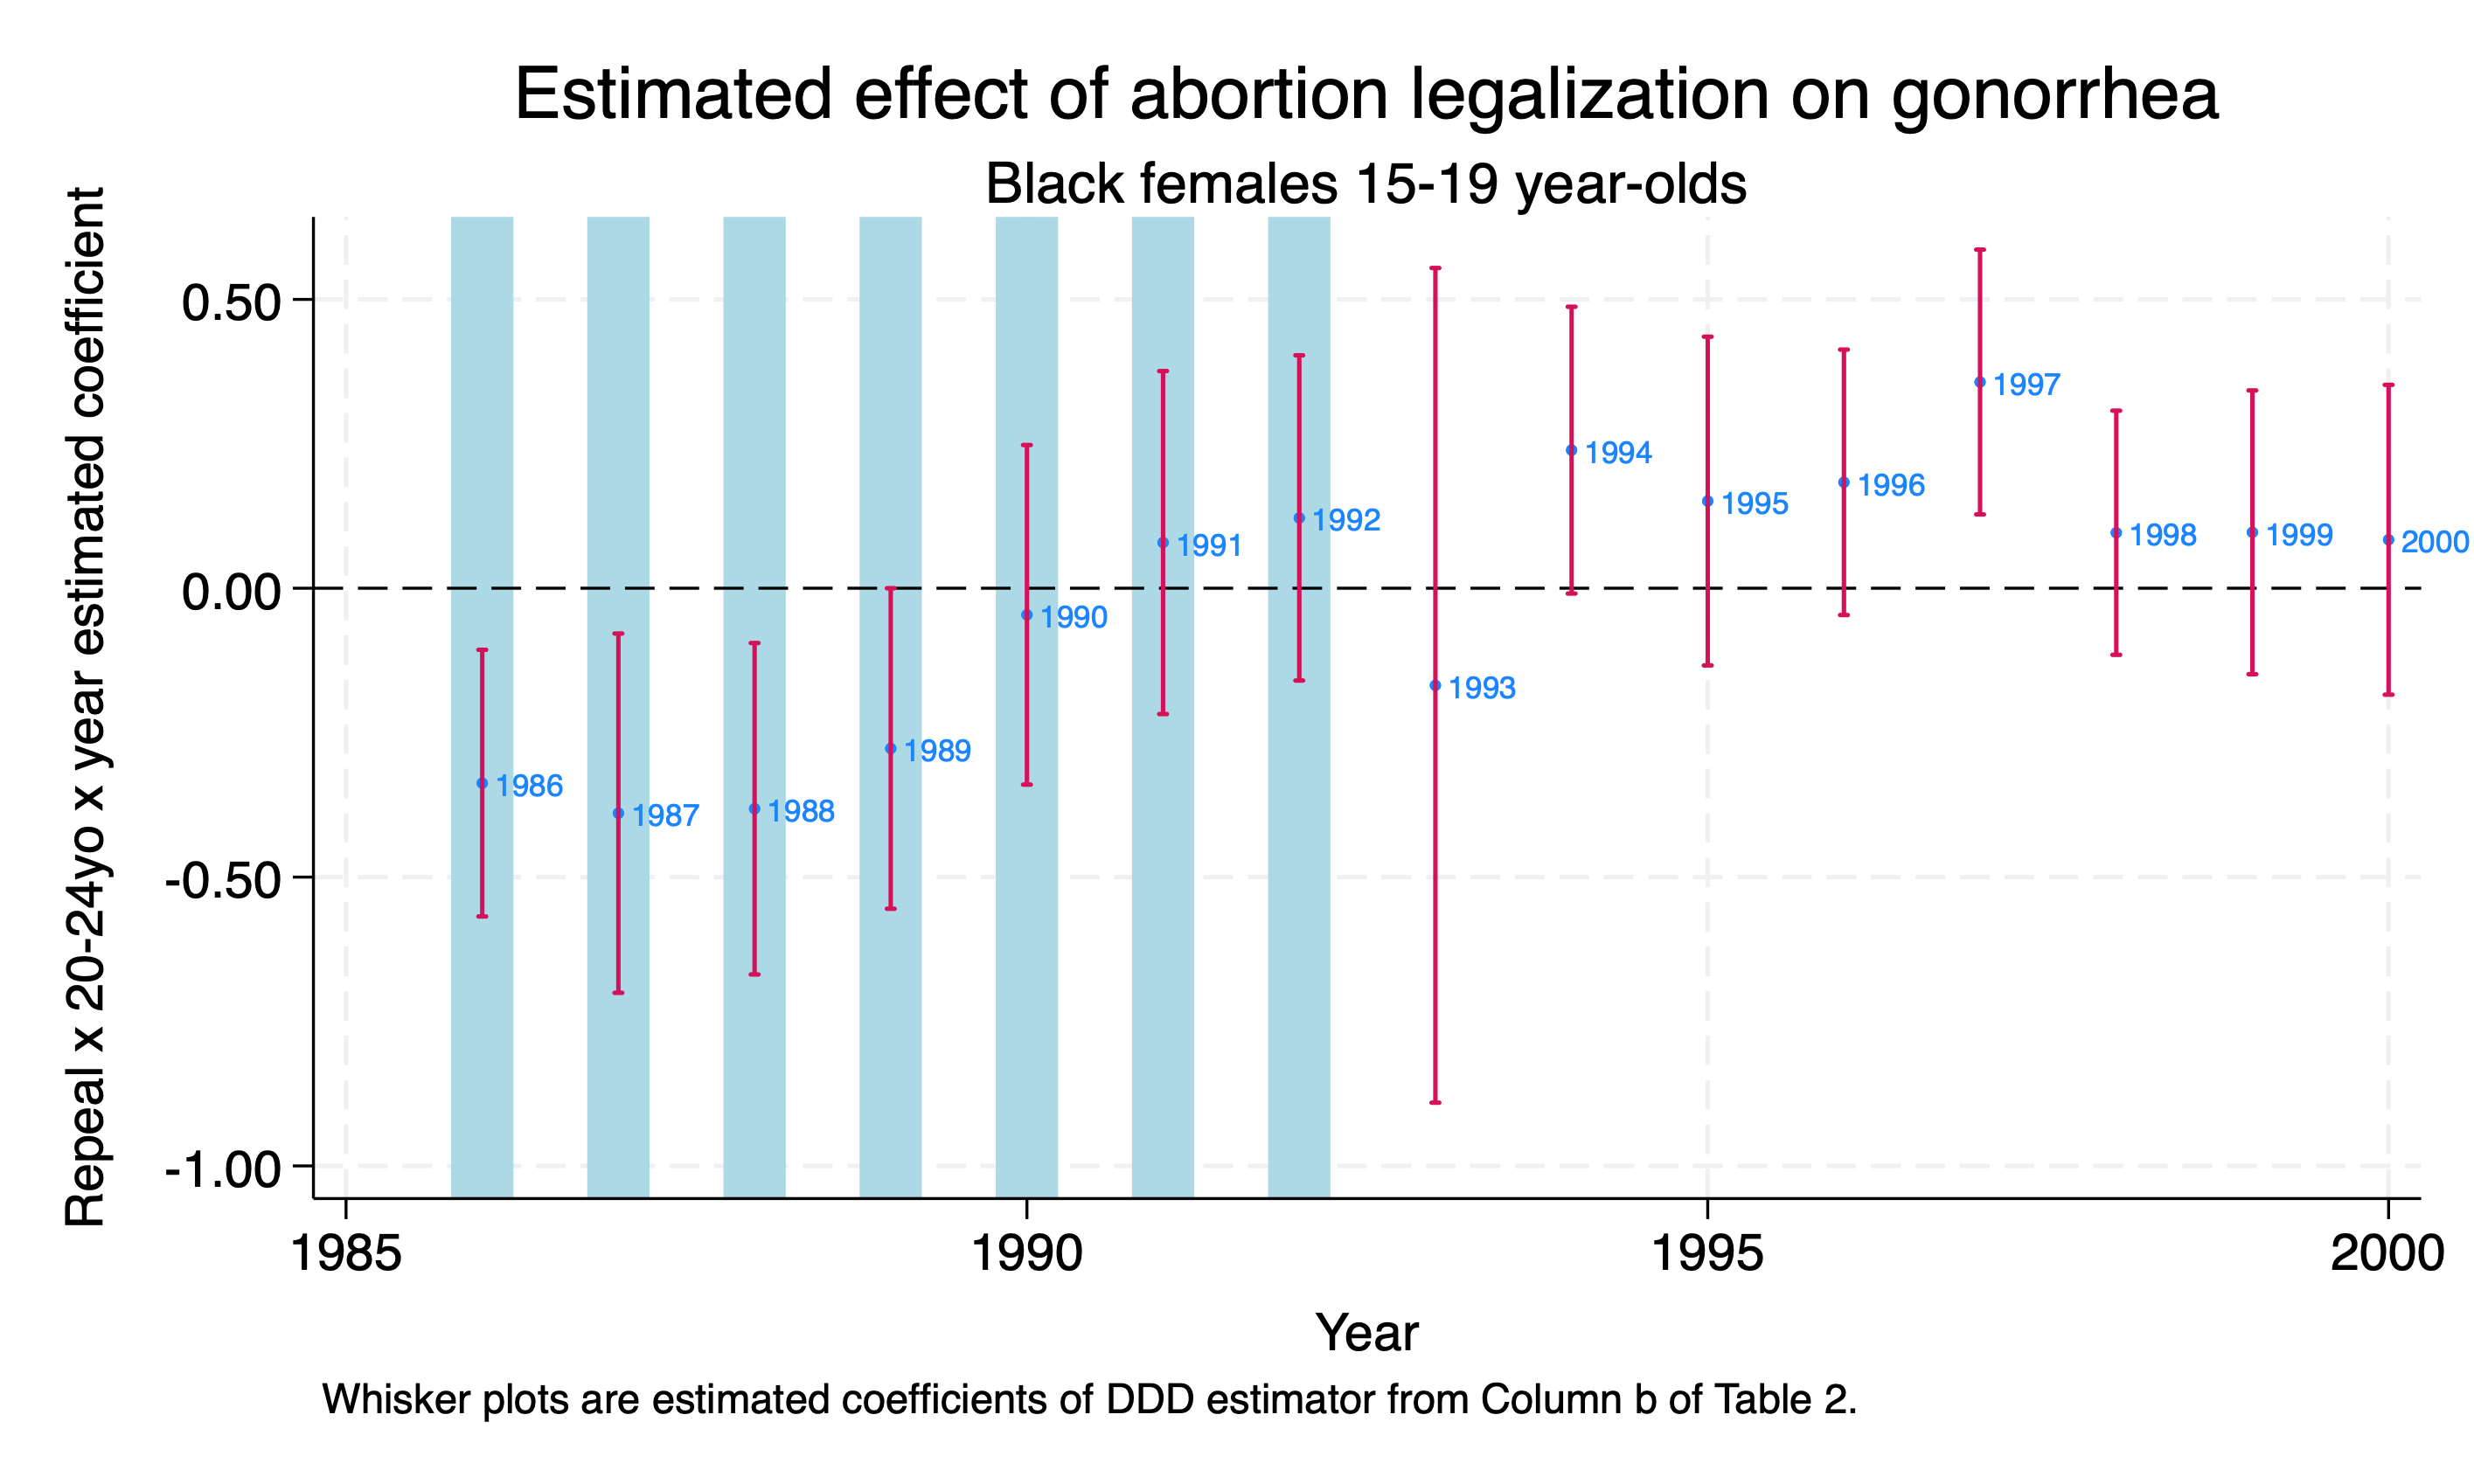
\includegraphics[keepaspectratio,alt={Parameter estimates for the DDD estimator for Black Females}]{DDD1.png}}
\caption{Parameter estimates for the DDD estimator for Black Females}
\end{figure}

It is interesting that we fail to reject the null hypothesis for 15-19 year olds in 1991-1992, but we reject the null hypothesis for 25-29 year olds in 1991-1992.

We can run the estimates for White women, Black males, and White males. The code is the same as above with the exception of the subset.

\begin{figure}
\centering
\pandocbounded{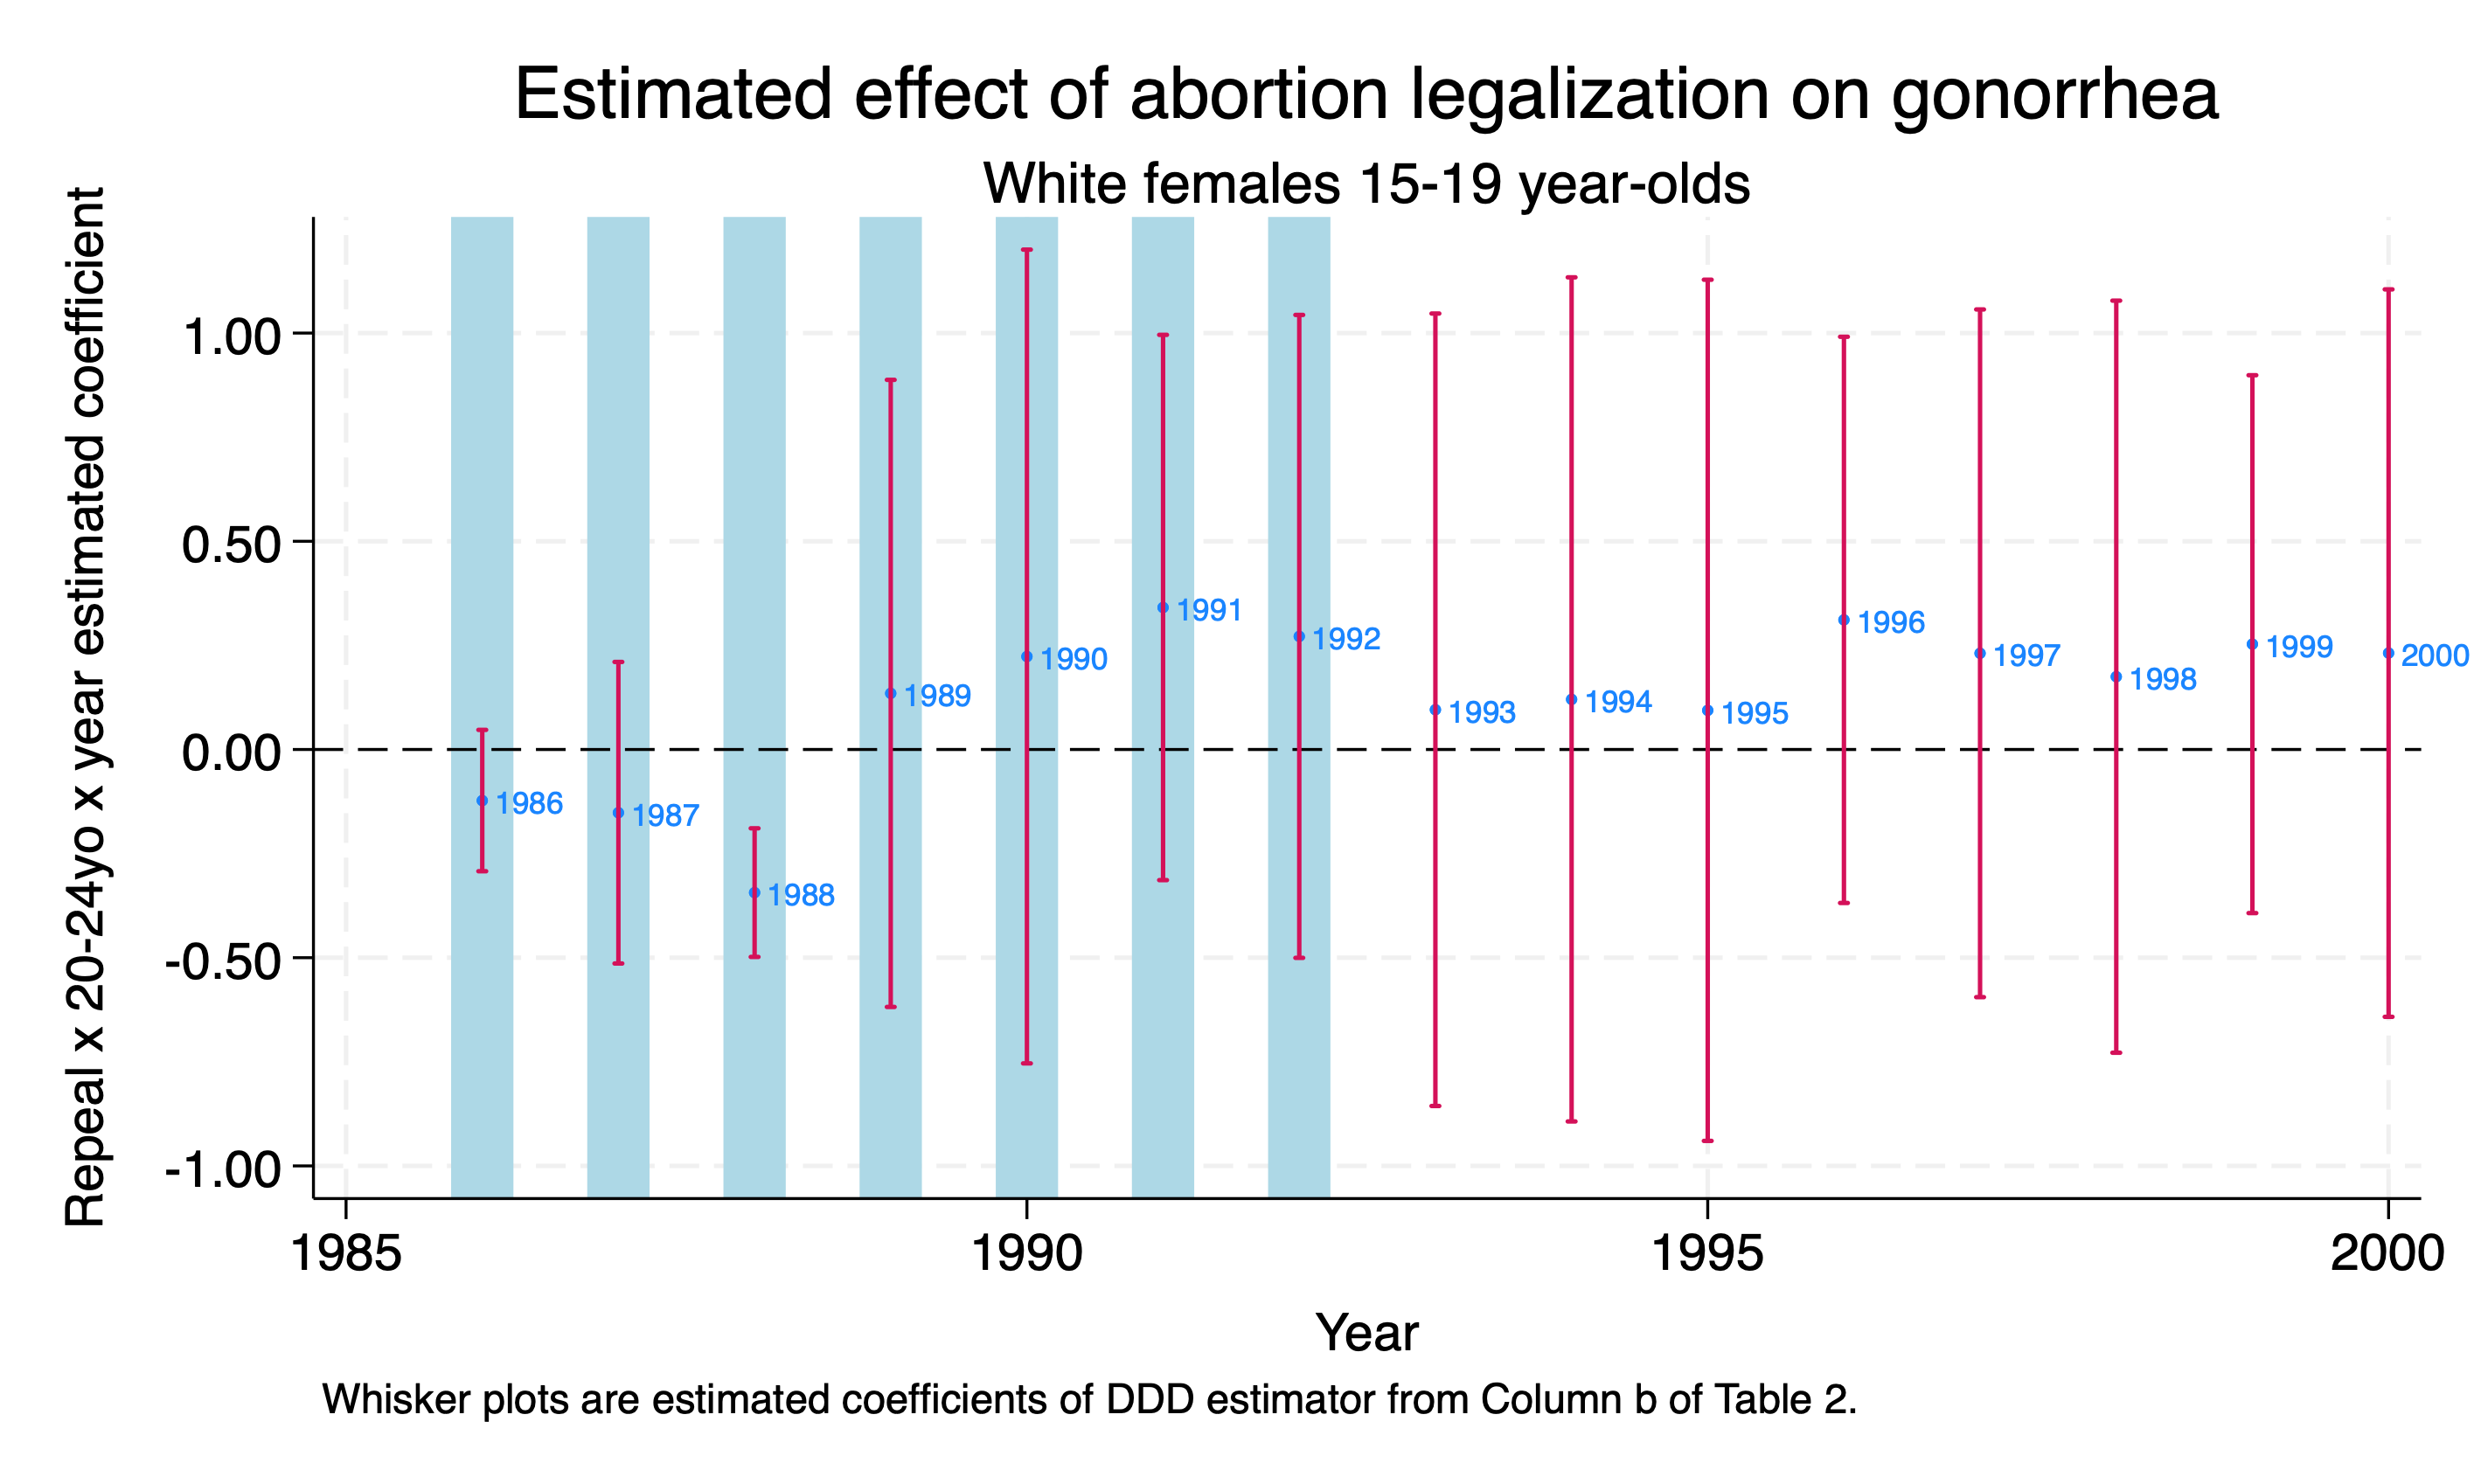
\includegraphics[keepaspectratio,alt={Parameter estimates for White Women}]{DDD2.png}}
\caption{Parameter estimates for White Women}
\end{figure}

We fail to reject the null hypothesis that parameters for the DDD estimator are 0 with the exception of 1988.

\begin{figure}
\centering
\pandocbounded{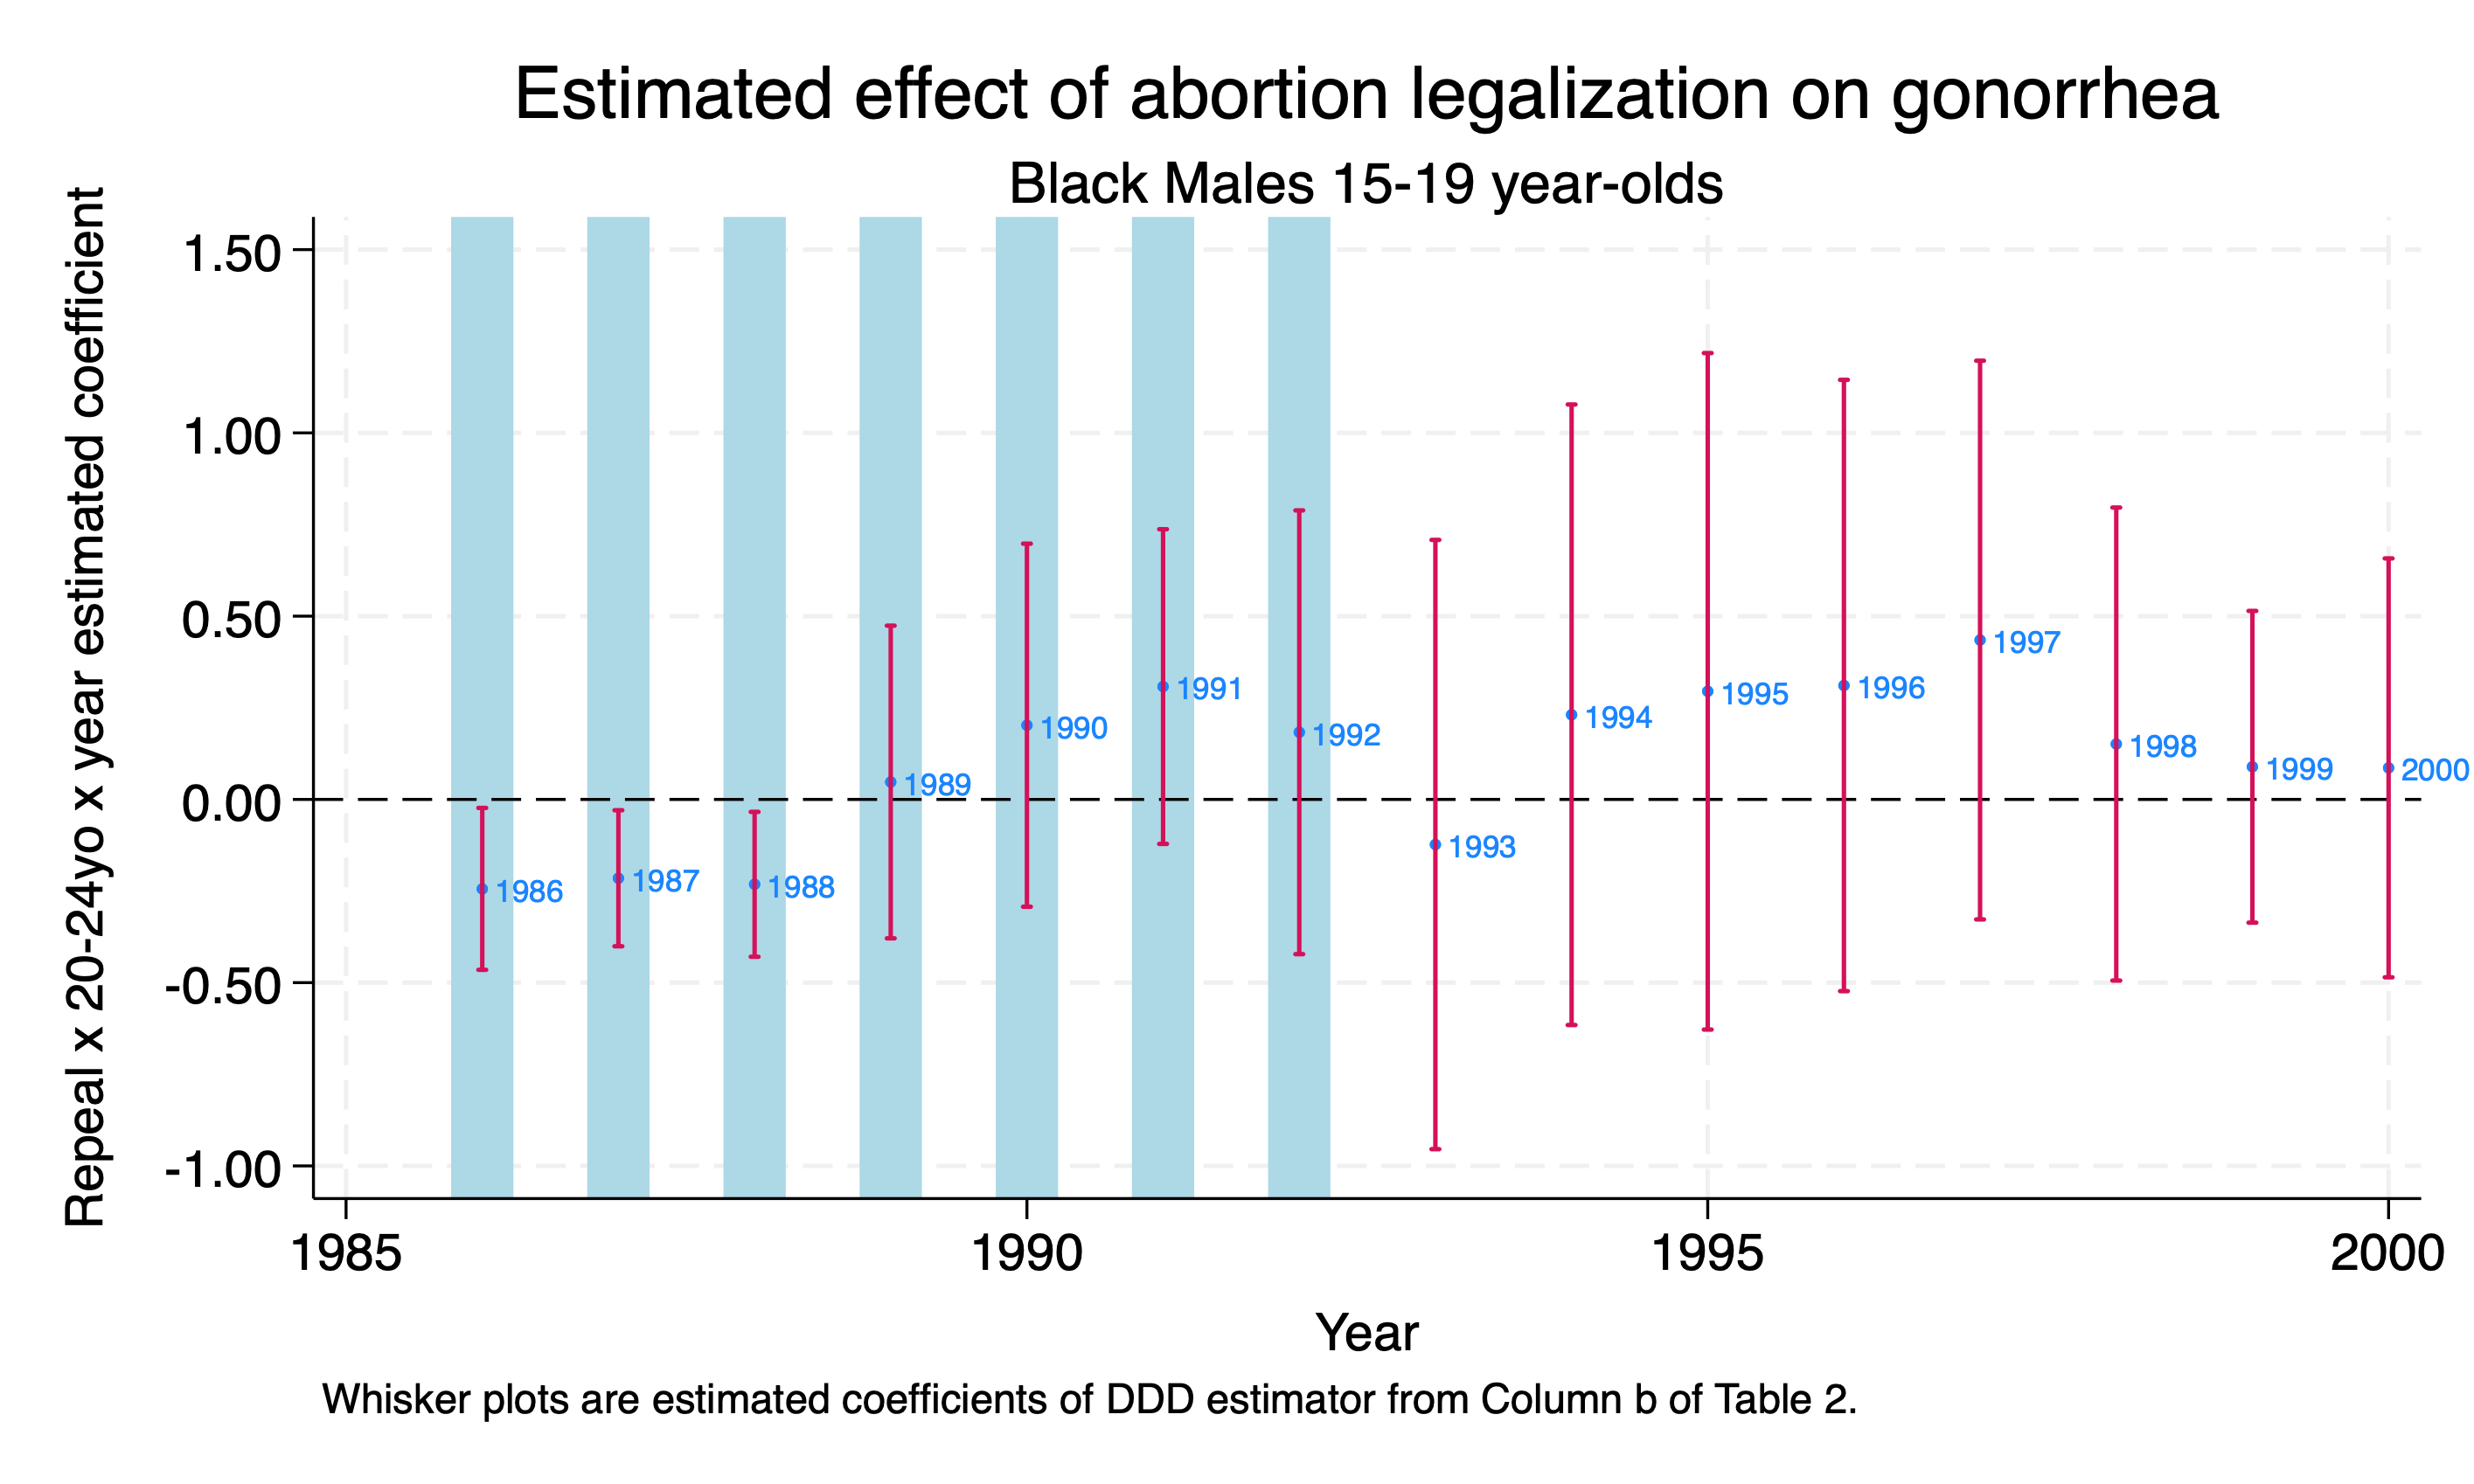
\includegraphics[keepaspectratio,alt={Parameter estimates for Black Males}]{DDD3.png}}
\caption{Parameter estimates for Black Males}
\end{figure}

We reject the null hypothesis that the parameters of the DDD estimator is 0 for 1986-1988, but we fail to reject the null hypothesis for years 1989-1992.

\begin{figure}
\centering
\pandocbounded{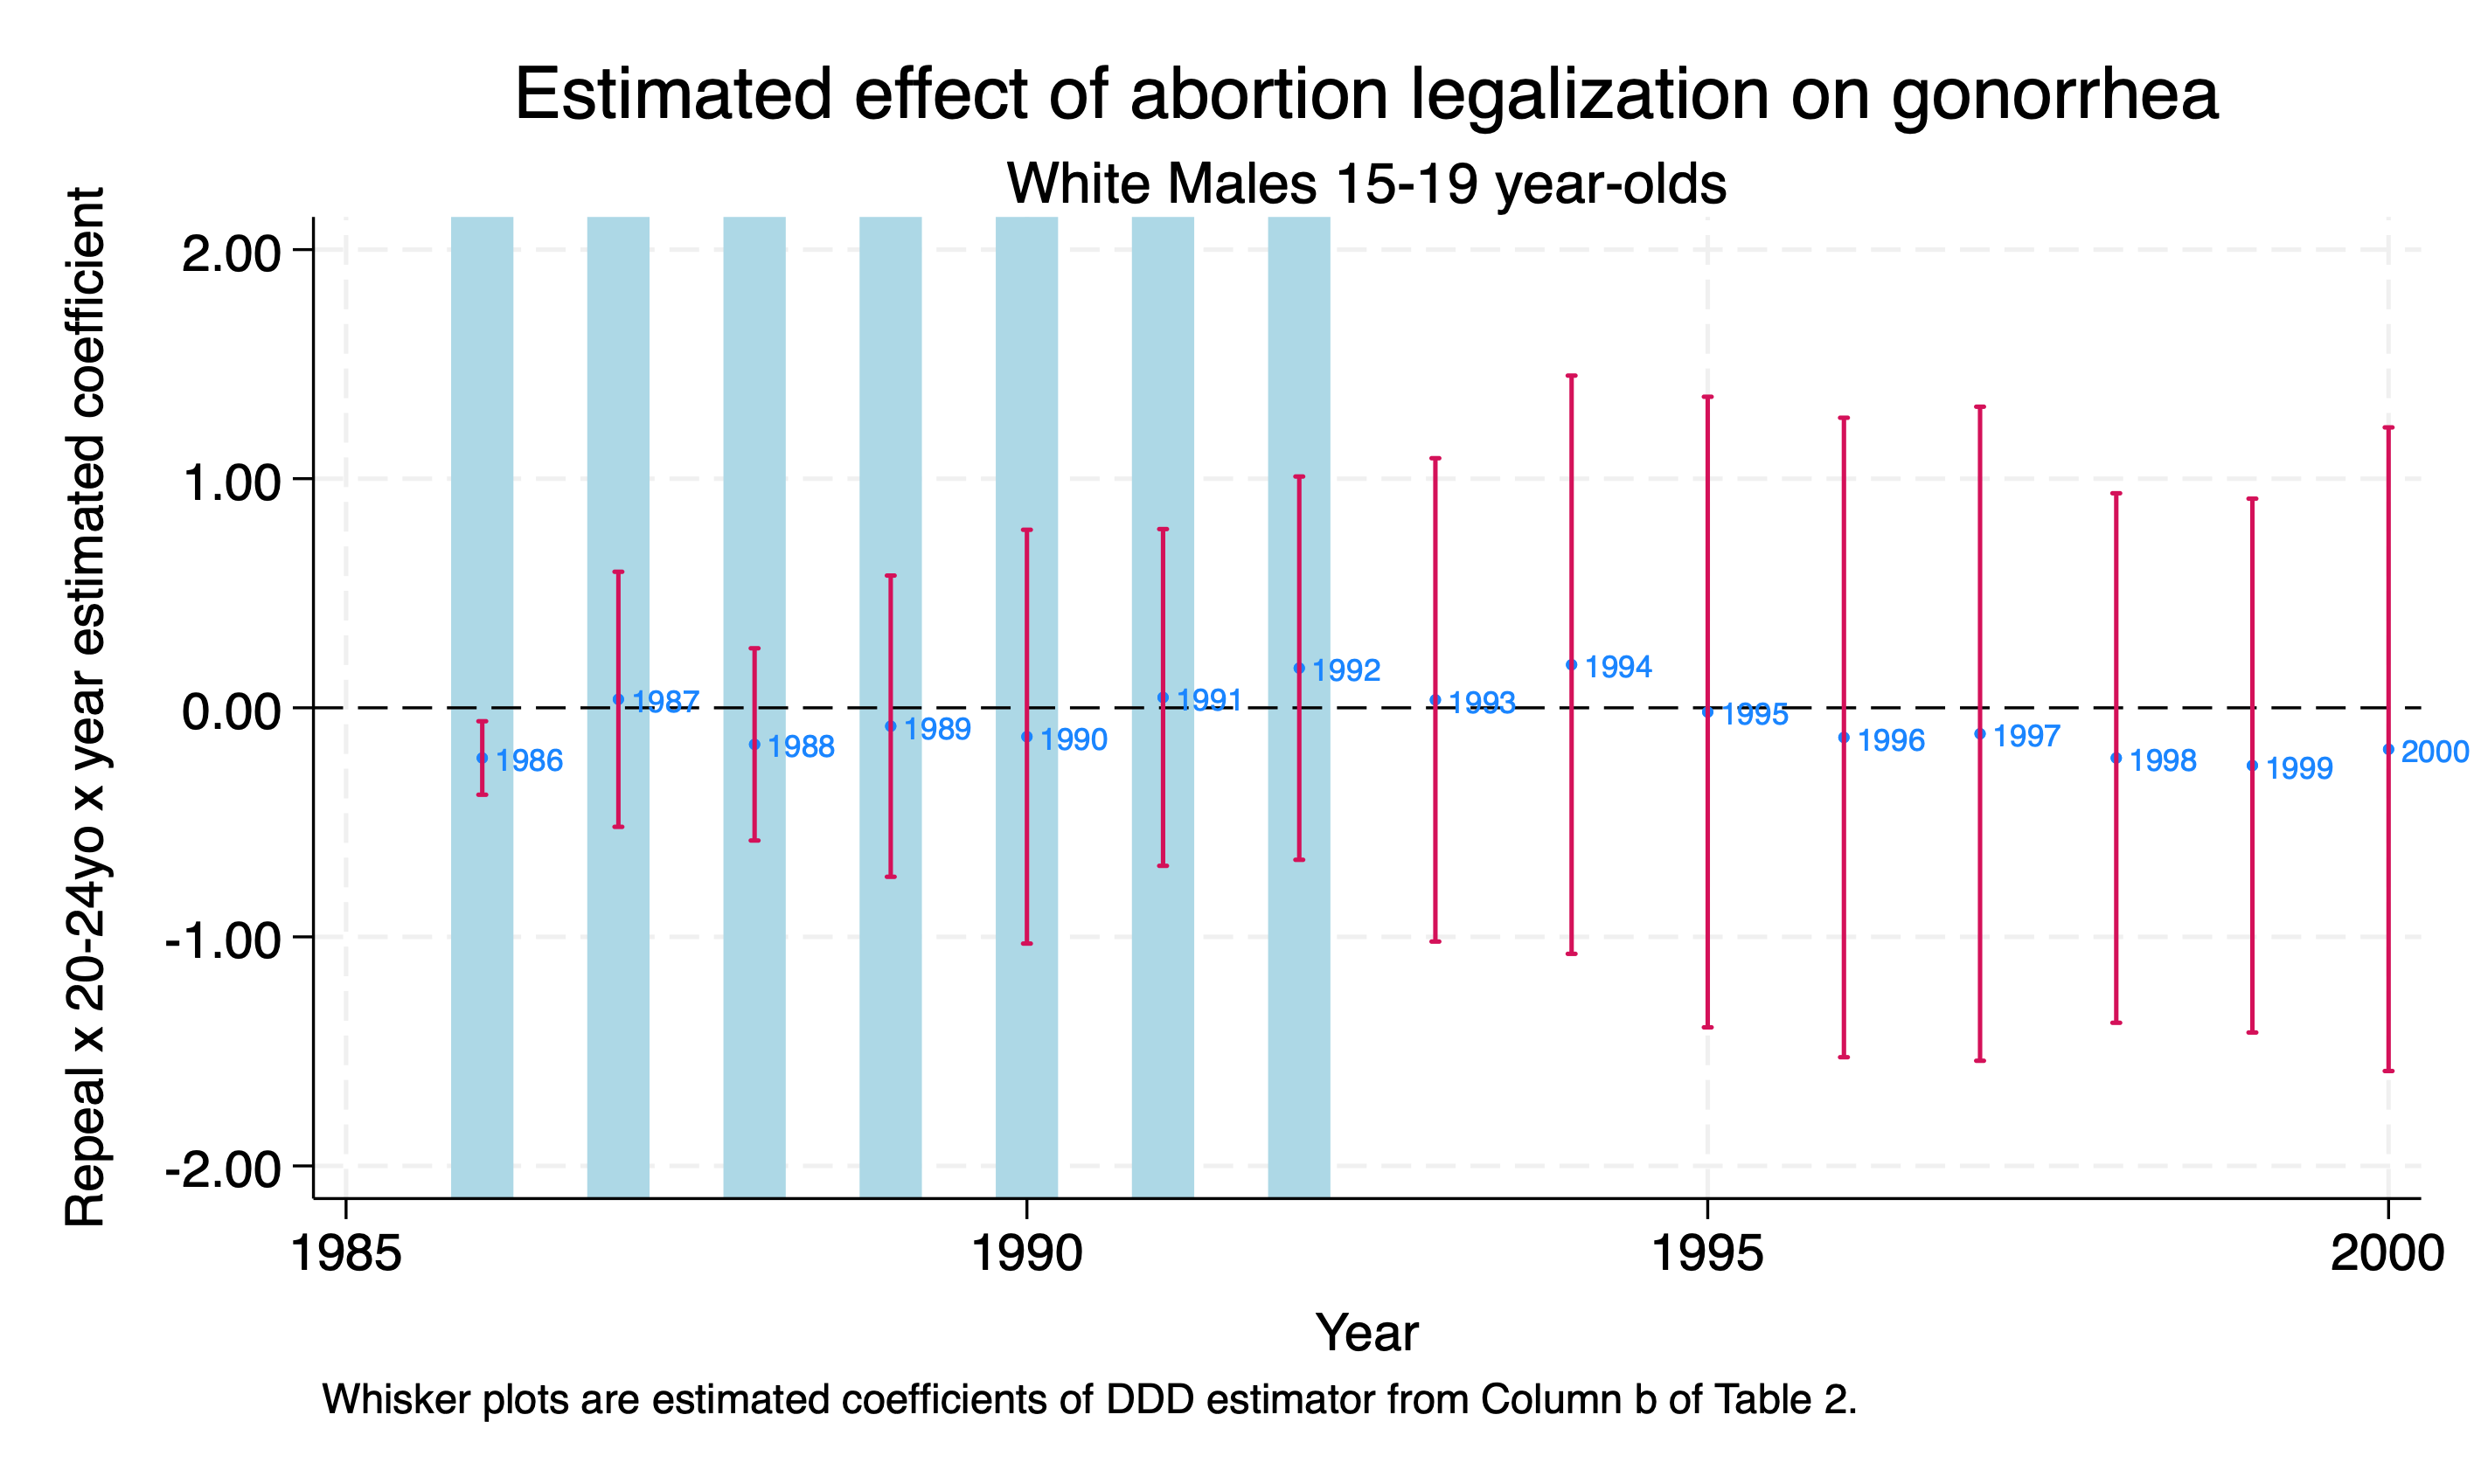
\includegraphics[keepaspectratio,alt={Parameter Estimates for White Males}]{DDD4.png}}
\caption{Parameter Estimates for White Males}
\end{figure}

We fail to reject the null hypothesis that the parameters of the DDD estimator are 0 for White Males, except for 1986.

These results show that the policy impacts may vary by demographics. However, these tests show some support to what Cunningham and Cornwell (2013) hypothesis. However, as Cunningham (2021) notes the abortion hypothesis makes very specific predictions, and we fail to find a parabolic relationship.

\section{20-24 year olds vs 25-29 year olds}\label{year-olds-vs-25-29-year-olds}

Next, we will conduct the same exercise, but we will focus on 20-24 year olds.

\begin{Shaded}
\begin{Highlighting}[]
\KeywordTok{quietly}\NormalTok{ \{}
\KeywordTok{use} \StringTok{"/Users/Sam/Desktop/Econ 672/Data/abortion.dta"}\NormalTok{, }\KeywordTok{clear}

\NormalTok{Second DDD }\KeywordTok{model} \KeywordTok{for}\NormalTok{ 20{-}24 }\FunctionTok{year}\NormalTok{ olds vs 25{-}29 }\FunctionTok{year}\NormalTok{ olds }\BaseNTok{black}\NormalTok{ females }\KeywordTok{in}\NormalTok{ repeal vs Roe states}
\KeywordTok{gen}\NormalTok{ younger2 = 0 }
\KeywordTok{replace}\NormalTok{ younger2 = 1 }\KeywordTok{if}\NormalTok{ age == 20}

\KeywordTok{gen}\NormalTok{ yr2=(repeal==1) \& (younger2==1)}

\KeywordTok{gen}\NormalTok{ wm=(wht==1) \& (male==1)}
\KeywordTok{gen}\NormalTok{ wf=(wht==1) \& (male==0)}
\KeywordTok{gen}\NormalTok{ bm=(wht==0) \& (male==1)}
\KeywordTok{gen}\NormalTok{ bf=(wht==0) \& (male==0)}
\FunctionTok{char} \FunctionTok{year}\NormalTok{[omit] 1985 }
\FunctionTok{char}\NormalTok{ repeal[omit] 0 }
\FunctionTok{char}\NormalTok{ younger2[omit] 0 }
\FunctionTok{char}\NormalTok{ fip[omit] 1 }
\FunctionTok{char}\NormalTok{ fa[omit] 0 }
\FunctionTok{char}\NormalTok{ yr2[omit] 0 }

\NormalTok{*Triple DDD }
\NormalTok{*Compare 20{-}24 to 25{-}29 }\FunctionTok{year}\NormalTok{ olds }\KeywordTok{in}\NormalTok{ repeal vs Roe states}
\NormalTok{*OR}
\KeywordTok{reg}\NormalTok{ lnr i.repeal\#\#i.year\#\#i.younger2 i.fip\#\#c.t acc }\KeywordTok{pi} \KeywordTok{ir}\NormalTok{ alcohol crack  poverty }\CommentTok{///}
\NormalTok{ income ur }\KeywordTok{if}\NormalTok{ bf==1 \& (age==20 | age==25) [}\KeywordTok{aweight}\NormalTok{=totpop], }\KeywordTok{cluster}\NormalTok{(fip) }
\NormalTok{*XI}
\KeywordTok{xi}\NormalTok{: }\KeywordTok{reg}\NormalTok{ lnr i.repeal*i.}\FunctionTok{year}\NormalTok{ i.younger2*i.repeal i.younger2*i.}\FunctionTok{year}\NormalTok{ i.yr2*i.}\FunctionTok{year} \CommentTok{///}
\NormalTok{  i.fip*t acc }\KeywordTok{pi} \KeywordTok{ir}\NormalTok{ alcohol crack  poverty income ur }\KeywordTok{if}\NormalTok{ bf==1 \& (age==20 | age==25) }\CommentTok{///}
\NormalTok{  [}\KeywordTok{aweight}\NormalTok{=totpop], }\KeywordTok{cluster}\NormalTok{(fip) }
  
\NormalTok{ parmest, }\KeywordTok{label} \KeywordTok{for}\NormalTok{(estimate min95 max95 \%8.2f) li(parm }\KeywordTok{label}\NormalTok{ estimate min95 max95) }\KeywordTok{saving}\NormalTok{(bf20\_DDD.dta, }\KeywordTok{replace}\NormalTok{)}

\NormalTok{*Get Parameter Estimate Dataframe}
\KeywordTok{use}\NormalTok{ ./bf20\_DDD.dta, }\KeywordTok{replace}

\KeywordTok{keep} \KeywordTok{in}\NormalTok{ 82/96}

\KeywordTok{gen}     \FunctionTok{year}\NormalTok{=.}
\KeywordTok{replace} \FunctionTok{year}\NormalTok{=1986 }\KeywordTok{in}\NormalTok{ 1}
\KeywordTok{replace} \FunctionTok{year}\NormalTok{=1987 }\KeywordTok{in}\NormalTok{ 2}
\KeywordTok{replace} \FunctionTok{year}\NormalTok{=1988 }\KeywordTok{in}\NormalTok{ 3}
\KeywordTok{replace} \FunctionTok{year}\NormalTok{=1989 }\KeywordTok{in}\NormalTok{ 4}
\KeywordTok{replace} \FunctionTok{year}\NormalTok{=1990 }\KeywordTok{in}\NormalTok{ 5}
\KeywordTok{replace} \FunctionTok{year}\NormalTok{=1991 }\KeywordTok{in}\NormalTok{ 6}
\KeywordTok{replace} \FunctionTok{year}\NormalTok{=1992 }\KeywordTok{in}\NormalTok{ 7}
\KeywordTok{replace} \FunctionTok{year}\NormalTok{=1993 }\KeywordTok{in}\NormalTok{ 8}
\KeywordTok{replace} \FunctionTok{year}\NormalTok{=1994 }\KeywordTok{in}\NormalTok{ 9}
\KeywordTok{replace} \FunctionTok{year}\NormalTok{=1995 }\KeywordTok{in}\NormalTok{ 10}
\KeywordTok{replace} \FunctionTok{year}\NormalTok{=1996 }\KeywordTok{in}\NormalTok{ 11}
\KeywordTok{replace} \FunctionTok{year}\NormalTok{=1997 }\KeywordTok{in}\NormalTok{ 12}
\KeywordTok{replace} \FunctionTok{year}\NormalTok{=1998 }\KeywordTok{in}\NormalTok{ 13}
\KeywordTok{replace} \FunctionTok{year}\NormalTok{=1999 }\KeywordTok{in}\NormalTok{ 14}
\KeywordTok{replace} \FunctionTok{year}\NormalTok{=2000 }\KeywordTok{in}\NormalTok{ 15}

\KeywordTok{sort} \FunctionTok{year}
\NormalTok{\}}
\NormalTok{*Graph the Triple Diff{-}}\KeywordTok{in}\NormalTok{{-}Diff}
\KeywordTok{twoway}\NormalTok{ (}\KeywordTok{scatter}\NormalTok{ estimate }\FunctionTok{year}\NormalTok{, }\BaseNTok{mlabel}\NormalTok{(}\FunctionTok{year}\NormalTok{) }\BaseNTok{mlabsize}\NormalTok{(vsmall) msize(tiny)) }\CommentTok{///}
\NormalTok{ (rcap min95 max95 }\FunctionTok{year}\NormalTok{, msize(vsmall)), }\CommentTok{///}
 \BaseNTok{ytitle}\NormalTok{(Repeal x 20{-}24yo x }\FunctionTok{year}\NormalTok{ estimated coefficient) }\BaseNTok{yscale}\NormalTok{(titlegap(2)) }\CommentTok{///}
 \KeywordTok{yline}\NormalTok{(0, lwidth(thin) lcolor(}\BaseNTok{black}\NormalTok{)) }\BaseNTok{xtitle}\NormalTok{(Year) }\CommentTok{///}
 \BaseNTok{xline}\NormalTok{(1991 1992 1993 1994 1995 1996 1997, lwidth(vvvthick) lpattern(solid) }\CommentTok{///}
\NormalTok{ lcolor(}\BaseNTok{ltblue}\NormalTok{)) }\BaseNTok{xscale}\NormalTok{(titlegap(2)) }\CommentTok{///}
 \BaseNTok{title}\NormalTok{(Estimated effect }\KeywordTok{of}\NormalTok{ abortion legalization }\KeywordTok{on}\NormalTok{ gonorrhea) }\CommentTok{///}
 \BaseNTok{subtitle}\NormalTok{(Black Females 20{-}24 }\FunctionTok{year}\NormalTok{{-}olds) }\CommentTok{///}
 \KeywordTok{note}\NormalTok{(Whisker plots are estimated coefficients }\KeywordTok{of}\NormalTok{ DDD estimator from Column b }\KeywordTok{of}\NormalTok{ Table 2.) }\CommentTok{///}
 \BaseNTok{legend}\NormalTok{(}\KeywordTok{off}\NormalTok{)}
\end{Highlighting}
\end{Shaded}

\begin{figure}
\centering
\pandocbounded{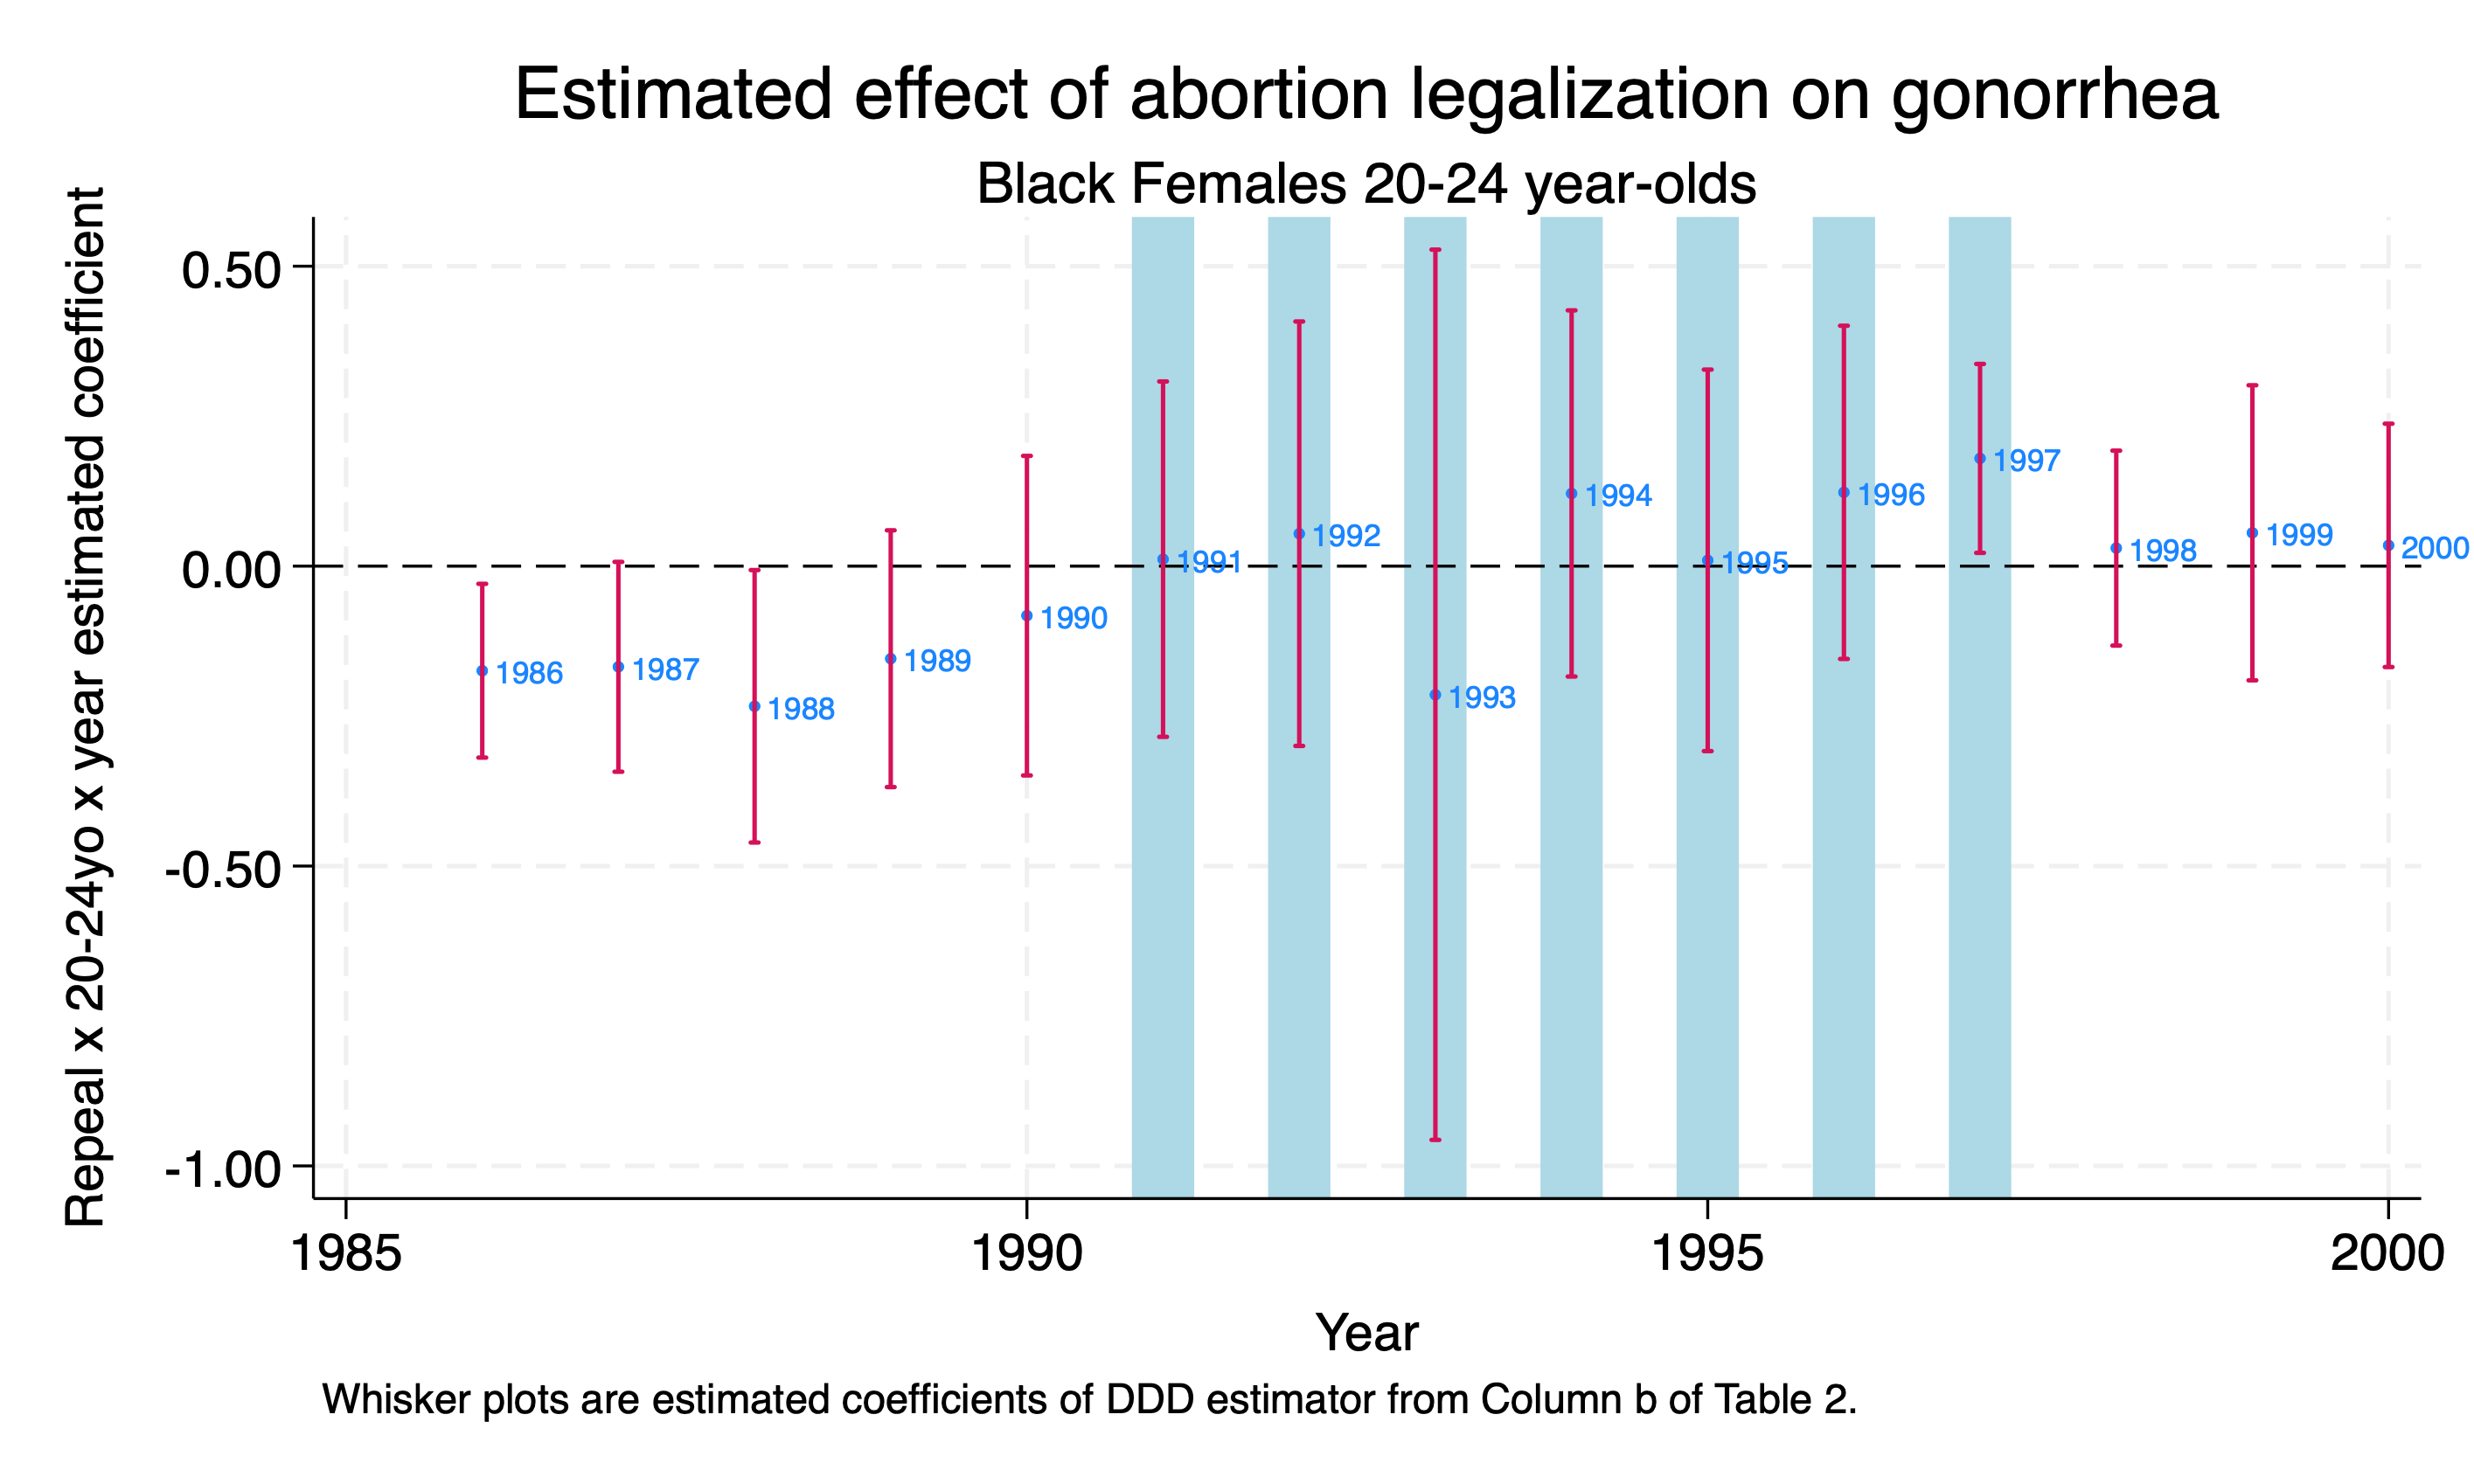
\includegraphics[keepaspectratio,alt={Parameter estimates for the DDD estimator for 20-24 Black Females}]{DDD5.png}}
\caption{Parameter estimates for the DDD estimator for 20-24 Black Females}
\end{figure}

We fail to reject the null hypothesis in the time period of interest. One concern is that 20-24 year olds are too close in age to 25-29 year olds for a comparison. If these groups are interacting, then we will have a spillover effect. This spillover effect will violate our Stable Unit Treatment Value Assumptions (SUTVA).

The abortion hypothesis provides very specific predictions, and our results show some skepticism for the abortion hypothesis explaining long-term gonorrehea incidences.

\chapter{Event Studies}\label{event-studies}

We can use panel event studies to assess pre-treatment trends. (Please do not confuse panel event studies with time series event studies). We will use data from the National Longitudinal Survey for Women to assess the impact of unionization on wages.

Luckily, we have some Stata commands that will help us with event studies. I have found these commands easier to use than the syntax provided by Cunningham (2021). Freyaldenhoven, Hansen, Perez, and Shapiro (2021) provide their command package \emph{xtevent} to estimate the parameters of an event study, plot the estimates, and test the estimates.

\begin{Shaded}
\begin{Highlighting}[]
\KeywordTok{ssc}\NormalTok{ install xtevent}
\end{Highlighting}
\end{Shaded}

\section{National Longitudinal Survey}\label{national-longitudinal-survey}

First, we will need to import the data and inspect the dataset.

\begin{Shaded}
\begin{Highlighting}[]
\NormalTok{cd }\StringTok{"/Users/Sam/Desktop/Econ 672/Data/"}
\KeywordTok{use}\NormalTok{ nlswork}

\KeywordTok{describe}
\end{Highlighting}
\end{Shaded}

\begin{verbatim}
/Users/Sam/Desktop/Econ 672/Data

(National Longitudinal Survey of Young Women, 14-24 years old in 1968)


Contains data from nlswork.dta
 Observations:        28,534                  National Longitudinal Survey of
                                                Young Women, 14-24 years old in
                                                1968
    Variables:            21                  13 Apr 2026 19:21
                                              (_dta has notes)
----------------------------------------------------------------------------------
Variable      Storage   Display    Value
    name         type    format    label      Variable label
----------------------------------------------------------------------------------
idcode          int     %8.0g                 NLS ID
year            byte    %8.0g                 Interview year
birth_yr        byte    %8.0g                 Birth year
age             byte    %8.0g                 Age in current year
race            byte    %8.0g      racelbl    Race
msp             byte    %8.0g                 1 if married, spouse present
nev_mar         byte    %8.0g                 1 if never married
grade           byte    %8.0g                 Current grade completed
collgrad        byte    %8.0g                 1 if college graduate
not_smsa        byte    %8.0g                 1 if not SMSA
c_city          byte    %8.0g                 1 if central city
south           byte    %8.0g                 1 if south
ind_code        byte    %8.0g                 Industry of employment
occ_code        byte    %8.0g                 Occupation
union           byte    %8.0g                 1 if union
wks_ue          byte    %8.0g                 Weeks unemployed last year
ttl_exp         float   %9.0g                 Total work experience
tenure          float   %9.0g                 Job tenure, in years
hours           int     %8.0g                 Usual hours worked
wks_work        int     %8.0g                 Weeks worked last year
ln_wage         float   %9.0g                 ln(wage/GNP deflator)
----------------------------------------------------------------------------------
Sorted by: idcode  year
\end{verbatim}

We can see that this is a longitudinal survey of women ages 14-24 in 1964. Let's inspect the outcome of interest, the natural log of wages.

\begin{Shaded}
\begin{Highlighting}[]
\KeywordTok{sum}\NormalTok{ ln\_wages, }\KeywordTok{detail}
\KeywordTok{histogram}\NormalTok{ ln\_wage, }\BaseNTok{title}\NormalTok{(Natural Log }\KeywordTok{of}\NormalTok{ Wages) }\BaseNTok{caption}\NormalTok{(NLS Women Ages 14{-}24 1964)}
\end{Highlighting}
\end{Shaded}

\begin{verbatim}
variable ln_wages not found
r(111);

r(111);
\end{verbatim}

\begin{figure}
\centering
\pandocbounded{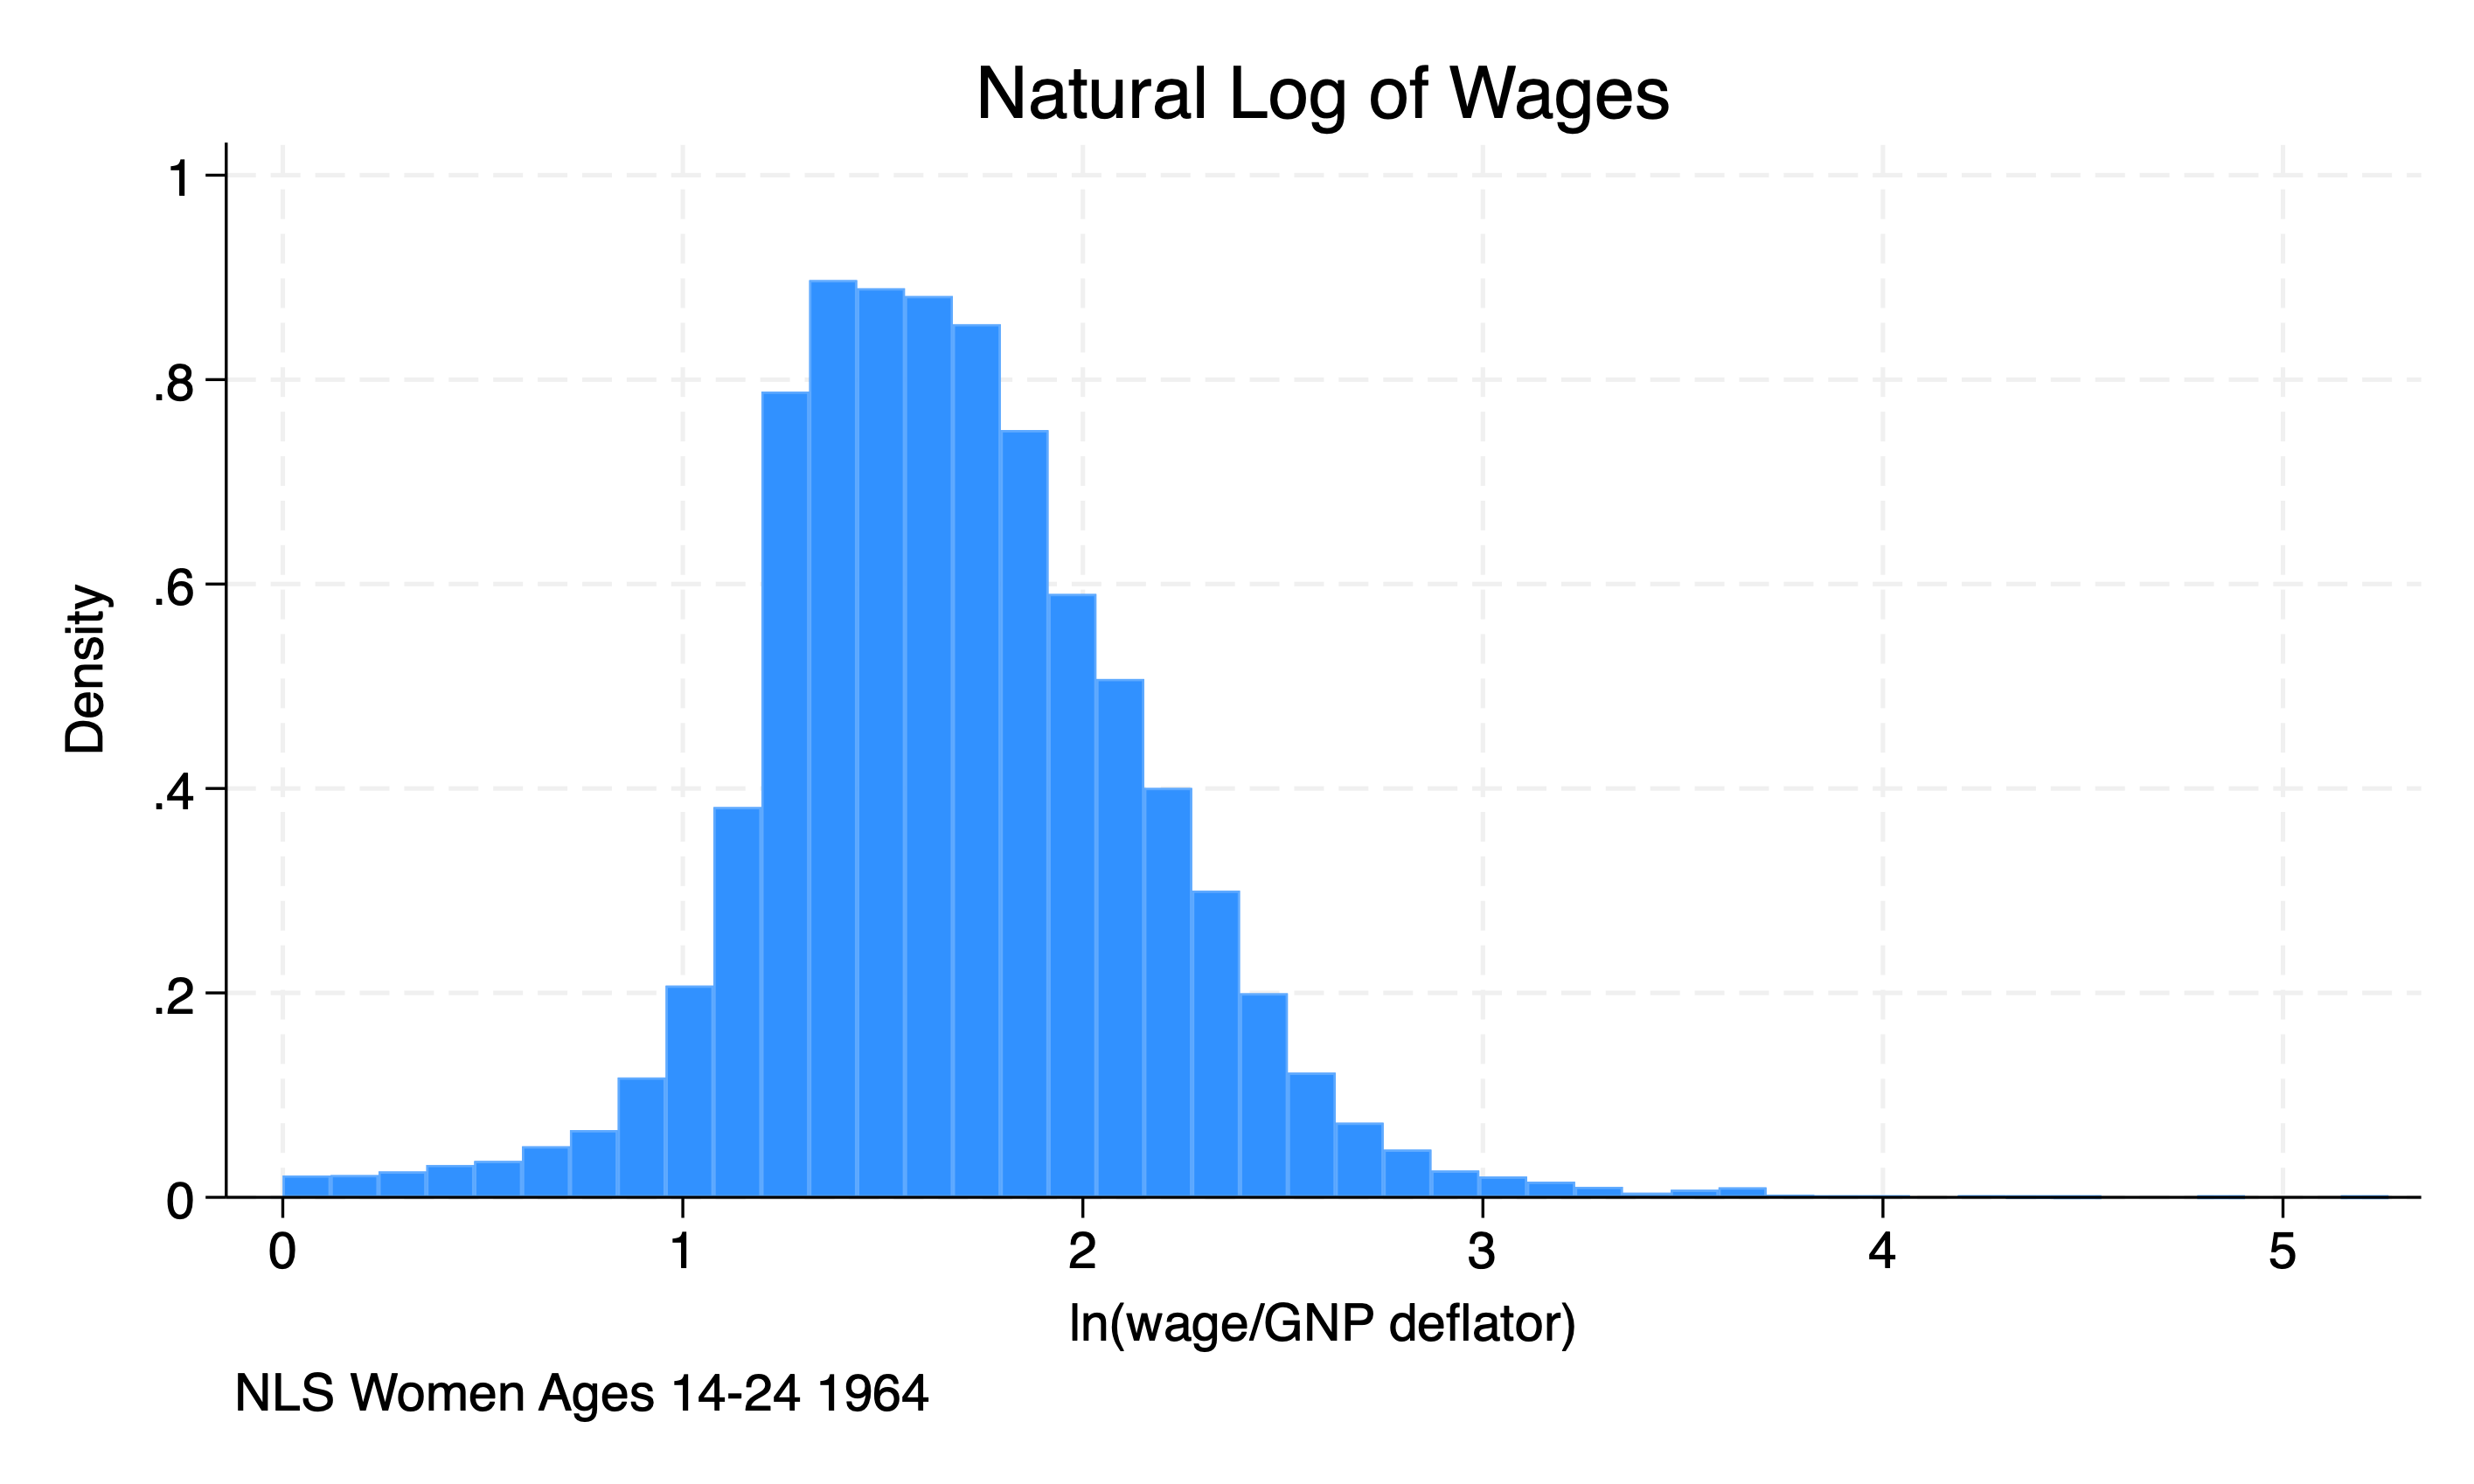
\includegraphics[keepaspectratio,alt={Histogram of Natural Log of Wages}]{ES1.png}}
\caption{Histogram of Natural Log of Wages}
\end{figure}

Next, we will set up the panel

\begin{Shaded}
\begin{Highlighting}[]
\KeywordTok{by}\NormalTok{ idcode (}\FunctionTok{year}\NormalTok{): }\KeywordTok{gen}\NormalTok{ time=}\DataTypeTok{\_n}
\NormalTok{xtset idcode time}
\end{Highlighting}
\end{Shaded}

\begin{verbatim}
Panel variable: idcode (unbalanced)
 Time variable: time, 1 to 15
         Delta: 1 unit
\end{verbatim}

Generate a policy variable that follows staggered adoption. This observe changes in the union status or treatment variable of interest.

\begin{Shaded}
\begin{Highlighting}[]
\KeywordTok{by}\NormalTok{ idcode (time): }\KeywordTok{gen}\NormalTok{ union2 = }\KeywordTok{sum}\NormalTok{(}\KeywordTok{union}\NormalTok{)}
\KeywordTok{replace}\NormalTok{ union2 = 1 }\KeywordTok{if}\NormalTok{ union2 \textgreater{} 1}
\KeywordTok{tab} \FunctionTok{year}\NormalTok{ union2}
\end{Highlighting}
\end{Shaded}

\begin{verbatim}
(4,177 real changes made)


 Interview |        union2
      year |         0          1 |     Total
-----------+----------------------+----------
        68 |     1,375          0 |     1,375 
        69 |     1,232          0 |     1,232 
        70 |     1,508        178 |     1,686 
        71 |     1,559        292 |     1,851 
        72 |     1,345        348 |     1,693 
        73 |     1,561        420 |     1,981 
        75 |     1,787        354 |     2,141 
        77 |     1,595        576 |     2,171 
        78 |     1,390        574 |     1,964 
        80 |     1,124        723 |     1,847 
        82 |     1,245        840 |     2,085 
        83 |     1,171        816 |     1,987 
        85 |     1,184        901 |     2,085 
        87 |     1,213        951 |     2,164 
        88 |     1,270      1,002 |     2,272 
-----------+----------------------+----------
     Total |    20,559      7,975 |    28,534 
\end{verbatim}

\section{\texorpdfstring{\emph{xtevent}}{xtevent}}\label{xtevent}

We can utilize the command \emph{xtevent} to calculate and plot an panel event study instead of complex syntax. The command is the following:

\textbf{xtevent} \emph{depvar} {[}\emph{indepvars}{]}, policyvar(\emph{PostTreatVar}) panelvar(\emph{idvar}) timevar(\emph{timevarname})

We have several options that we need to consider as well. One of the key option is the \emph{window} options. We will set the window to 3 and then rerun the \emph{xtevent} command with a window of 10.

\begin{Shaded}
\begin{Highlighting}[]
\NormalTok{xtevent ln\_w age c.age\#c.age ttl\_exp c.ttl\_exp\#c.ttl\_exp tenure , pol(union2) }\FunctionTok{w}\NormalTok{(3) }\KeywordTok{cluster}\NormalTok{(idcode) }\KeywordTok{impute}\NormalTok{(nuchange)}
\end{Highlighting}
\end{Shaded}

\begin{verbatim}
Using options panelvar and timevar from xtset

No proxy or instruments provided. Implementing OLS estimator

Linear regression, absorbing indicators             Number of obs     = 23,541
Absorbed variable: idcode                           No. of categories =  2,771
                                                    F(27, 2770)       =  68.03
                                                    Prob > F          = 0.0000
                                                    R-squared         = 0.6662
                                                    Adj R-squared     = 0.6212
                                                    Root MSE          = 0.2872

                             (Std. err. adjusted for 2,771 clusters in idcode)
------------------------------------------------------------------------------
             |               Robust
     ln_wage | Coefficient  std. err.      t    P>|t|     [95% conf. interval]
-------------+----------------------------------------------------------------
    _k_eq_m4 |  -.0449924   .0184471    -2.44   0.015    -.0811639   -.0088209
    _k_eq_m3 |  -.0565855   .0168862    -3.35   0.001    -.0896964   -.0234746
    _k_eq_m2 |  -.0421016   .0134889    -3.12   0.002    -.0685508   -.0156524
    _k_eq_p0 |    .089023   .0116097     7.67   0.000     .0662585    .1117874
    _k_eq_p1 |   .0815659   .0138364     5.90   0.000     .0544352    .1086966
    _k_eq_p2 |   .0804259   .0153595     5.24   0.000     .0503086    .1105431
    _k_eq_p3 |   .0635638   .0172566     3.68   0.000     .0297266     .097401
    _k_eq_p4 |   .0299474   .0202315     1.48   0.139    -.0097229    .0696178
         age |   .0200353   .0067278     2.98   0.003     .0068434    .0332273
             |
 c.age#c.age |  -.0005226   .0001023    -5.11   0.000    -.0007231    -.000322
             |
     ttl_exp |   .0491603   .0054054     9.09   0.000     .0385614    .0597593
             |
   c.ttl_exp#|
   c.ttl_exp |  -.0004479    .000193    -2.32   0.020    -.0008264   -.0000695
             |
      tenure |   .0095845   .0015872     6.04   0.000     .0064723    .0126967
             |
        time |
          2  |   .0560166   .0088315     6.34   0.000     .0386996    .0733335
          3  |   .0575122   .0129664     4.44   0.000     .0320874     .082937
          4  |   .0603109   .0171093     3.53   0.000     .0267627    .0938592
          5  |   .0485817   .0215347     2.26   0.024     .0063561    .0908074
          6  |   .0484417   .0263678     1.84   0.066    -.0032608    .1001441
          7  |   .0293154     .03143     0.93   0.351    -.0323131    .0909439
          8  |    .021307   .0362073     0.59   0.556    -.0496891    .0923031
          9  |   .0151769   .0409211     0.37   0.711    -.0650621    .0954159
         10  |  -.0014045    .045488    -0.03   0.975    -.0905984    .0877894
         11  |  -.0124446   .0507805    -0.25   0.806     -.112016    .0871269
         12  |  -.0173009   .0561008    -0.31   0.758    -.1273046    .0927028
         13  |  -.0346925   .0608558    -0.57   0.569    -.1540199    .0846348
         14  |  -.0097838   .0668818    -0.15   0.884     -.140927    .1213595
         15  |  -.0288719   .0799116    -0.36   0.718    -.1855643    .1278204
             |
       _cons |   1.221736   .1016406    12.02   0.000     1.022437    1.421035
------------------------------------------------------------------------------
\end{verbatim}

From the event study, we find that unionization increases wages for women by \((e^{0.089}-1)*100\% = 9.8\%\) to about \((e^{0.06356}-1)*100\% = 6.6\%\) for four years after unionization.

Now, we will expand the window to 10 years.

\begin{Shaded}
\begin{Highlighting}[]
\NormalTok{xtevent ln\_w age c.age\#c.age ttl\_exp c.ttl\_exp\#c.ttl\_exp tenure , pol(union2) }\FunctionTok{w}\NormalTok{(10) }\KeywordTok{cluster}\NormalTok{(idcode) }\KeywordTok{impute}\NormalTok{(nuchange)}
\end{Highlighting}
\end{Shaded}

\begin{verbatim}
Using options panelvar and timevar from xtset

No proxy or instruments provided. Implementing OLS estimator

Linear regression, absorbing indicators             Number of obs     =  6,687
Absorbed variable: idcode                           No. of categories =    510
                                                    F(41, 509)        =  18.19
                                                    Prob > F          = 0.0000
                                                    R-squared         = 0.6709
                                                    Adj R-squared     = 0.6414
                                                    Root MSE          = 0.2626

                               (Std. err. adjusted for 510 clusters in idcode)
------------------------------------------------------------------------------
             |               Robust
     ln_wage | Coefficient  std. err.      t    P>|t|     [95% conf. interval]
-------------+----------------------------------------------------------------
   _k_eq_m11 |  -.0935686   .0915262    -1.02   0.307    -.2733842     .086247
   _k_eq_m10 |  -.0700651   .0749131    -0.94   0.350     -.217242    .0771118
    _k_eq_m9 |   -.052819   .0531611    -0.99   0.321    -.1572612    .0516232
    _k_eq_m8 |  -.0481707   .0461557    -1.04   0.297    -.1388498    .0425083
    _k_eq_m7 |  -.0709862   .0420374    -1.69   0.092    -.1535744    .0116021
    _k_eq_m6 |  -.0815994   .0394746    -2.07   0.039    -.1591527   -.0040462
    _k_eq_m5 |  -.0735276   .0330956    -2.22   0.027    -.1385483   -.0085069
    _k_eq_m4 |  -.0792023   .0321908    -2.46   0.014    -.1424454   -.0159591
    _k_eq_m3 |   -.066719   .0278508    -2.40   0.017    -.1214358   -.0120023
    _k_eq_m2 |  -.0458597   .0243467    -1.88   0.060    -.0936922    .0019727
    _k_eq_p0 |   .0820767   .0208546     3.94   0.000      .041105    .1230485
    _k_eq_p1 |   .0836871   .0229813     3.64   0.000     .0385372    .1288369
    _k_eq_p2 |   .0760776   .0248914     3.06   0.002      .027175    .1249802
    _k_eq_p3 |   .0453932    .027055     1.68   0.094    -.0077599    .0985464
    _k_eq_p4 |   .0314656   .0335141     0.94   0.348    -.0343774    .0973086
    _k_eq_p5 |   .0592412   .0330584     1.79   0.074    -.0057065    .1241889
    _k_eq_p6 |   .0298114   .0366003     0.81   0.416    -.0420949    .1017177
    _k_eq_p7 |   .0346491   .0409492     0.85   0.398    -.0458012    .1150995
    _k_eq_p8 |   .0318303   .0456673     0.70   0.486    -.0578893    .1215499
    _k_eq_p9 |   .0263062   .0526183     0.50   0.617    -.0770695     .129682
   _k_eq_p10 |   .0151391   .0553342     0.27   0.785    -.0935724    .1238507
   _k_eq_p11 |   .0007066   .0605004     0.01   0.991    -.1181547     .119568
         age |   .0287481   .0175581     1.64   0.102    -.0057472    .0632434
             |
 c.age#c.age |  -.0008166   .0002452    -3.33   0.001    -.0012984   -.0003349
             |
     ttl_exp |   .0506316   .0107874     4.69   0.000     .0294383    .0718249
             |
   c.ttl_exp#|
   c.ttl_exp |  -.0003699   .0003314    -1.12   0.265     -.001021    .0002812
             |
      tenure |   .0062955    .002426     2.60   0.010     .0015294    .0110616
             |
        time |
          2  |   .0701101    .018315     3.83   0.000     .0341277    .1060924
          3  |   .0573137   .0288765     1.98   0.048     .0005819    .1140455
          4  |   .0617034    .039705     1.55   0.121    -.0163024    .1397092
          5  |   .0600686   .0524503     1.15   0.253    -.0429772    .1631144
          6  |   .0695395   .0659455     1.05   0.292    -.0600194    .1990985
          7  |   .0525483   .0821128     0.64   0.522    -.1087734      .21387
          8  |   .0604927   .0978685     0.62   0.537    -.1317833    .2527686
          9  |   .0688636   .1110785     0.62   0.536    -.1493652    .2870925
         10  |   .0520036    .127703     0.41   0.684    -.1988862    .3028935
         11  |   .0646191    .144279     0.45   0.654    -.2188365    .3480747
         12  |   .0959642   .1585038     0.61   0.545     -.215438    .4073664
         13  |   .1001231   .1730002     0.58   0.563    -.2397593    .4400056
         14  |   .1470231   .1898777     0.77   0.439    -.2260174    .5200636
         15  |   .1433274   .2071761     0.69   0.489    -.2636981    .5503529
             |
       _cons |   1.223692   .2833243     4.32   0.000     .6670628    1.780321
------------------------------------------------------------------------------
\end{verbatim}

We can see the range of outcomes is similar, but for only three years after the event.

\section{\texorpdfstring{\emph{xteventplot}}{xteventplot}}\label{xteventplot}

We can plot the results from the \emph{xtevent} command in two ways. One way is to add the option \emph{plot} to the \emph{xtevent} command. The second way is to use the command \emph{xteventplot}, which I prefer due to more options.

We can visualize the pretreatment trends to see if parallel trends holds.

\begin{Shaded}
\begin{Highlighting}[]
\KeywordTok{quietly}\NormalTok{ xtevent ln\_w age c.age\#c.age ttl\_exp c.ttl\_exp\#c.ttl\_exp tenure , pol(union2) }\FunctionTok{w}\NormalTok{(3) }\KeywordTok{cluster}\NormalTok{(idcode) }\KeywordTok{impute}\NormalTok{(nuchange) plot}

\NormalTok{xteventplot, }\BaseNTok{title}\NormalTok{(}\StringTok{"Event Study of Unionization on Wages"}\NormalTok{) }\BaseNTok{caption}\NormalTok{(}\StringTok{"NLS Women 14{-}24 in 1964"")}
\end{Highlighting}
\end{Shaded}

\begin{figure}
\centering
\pandocbounded{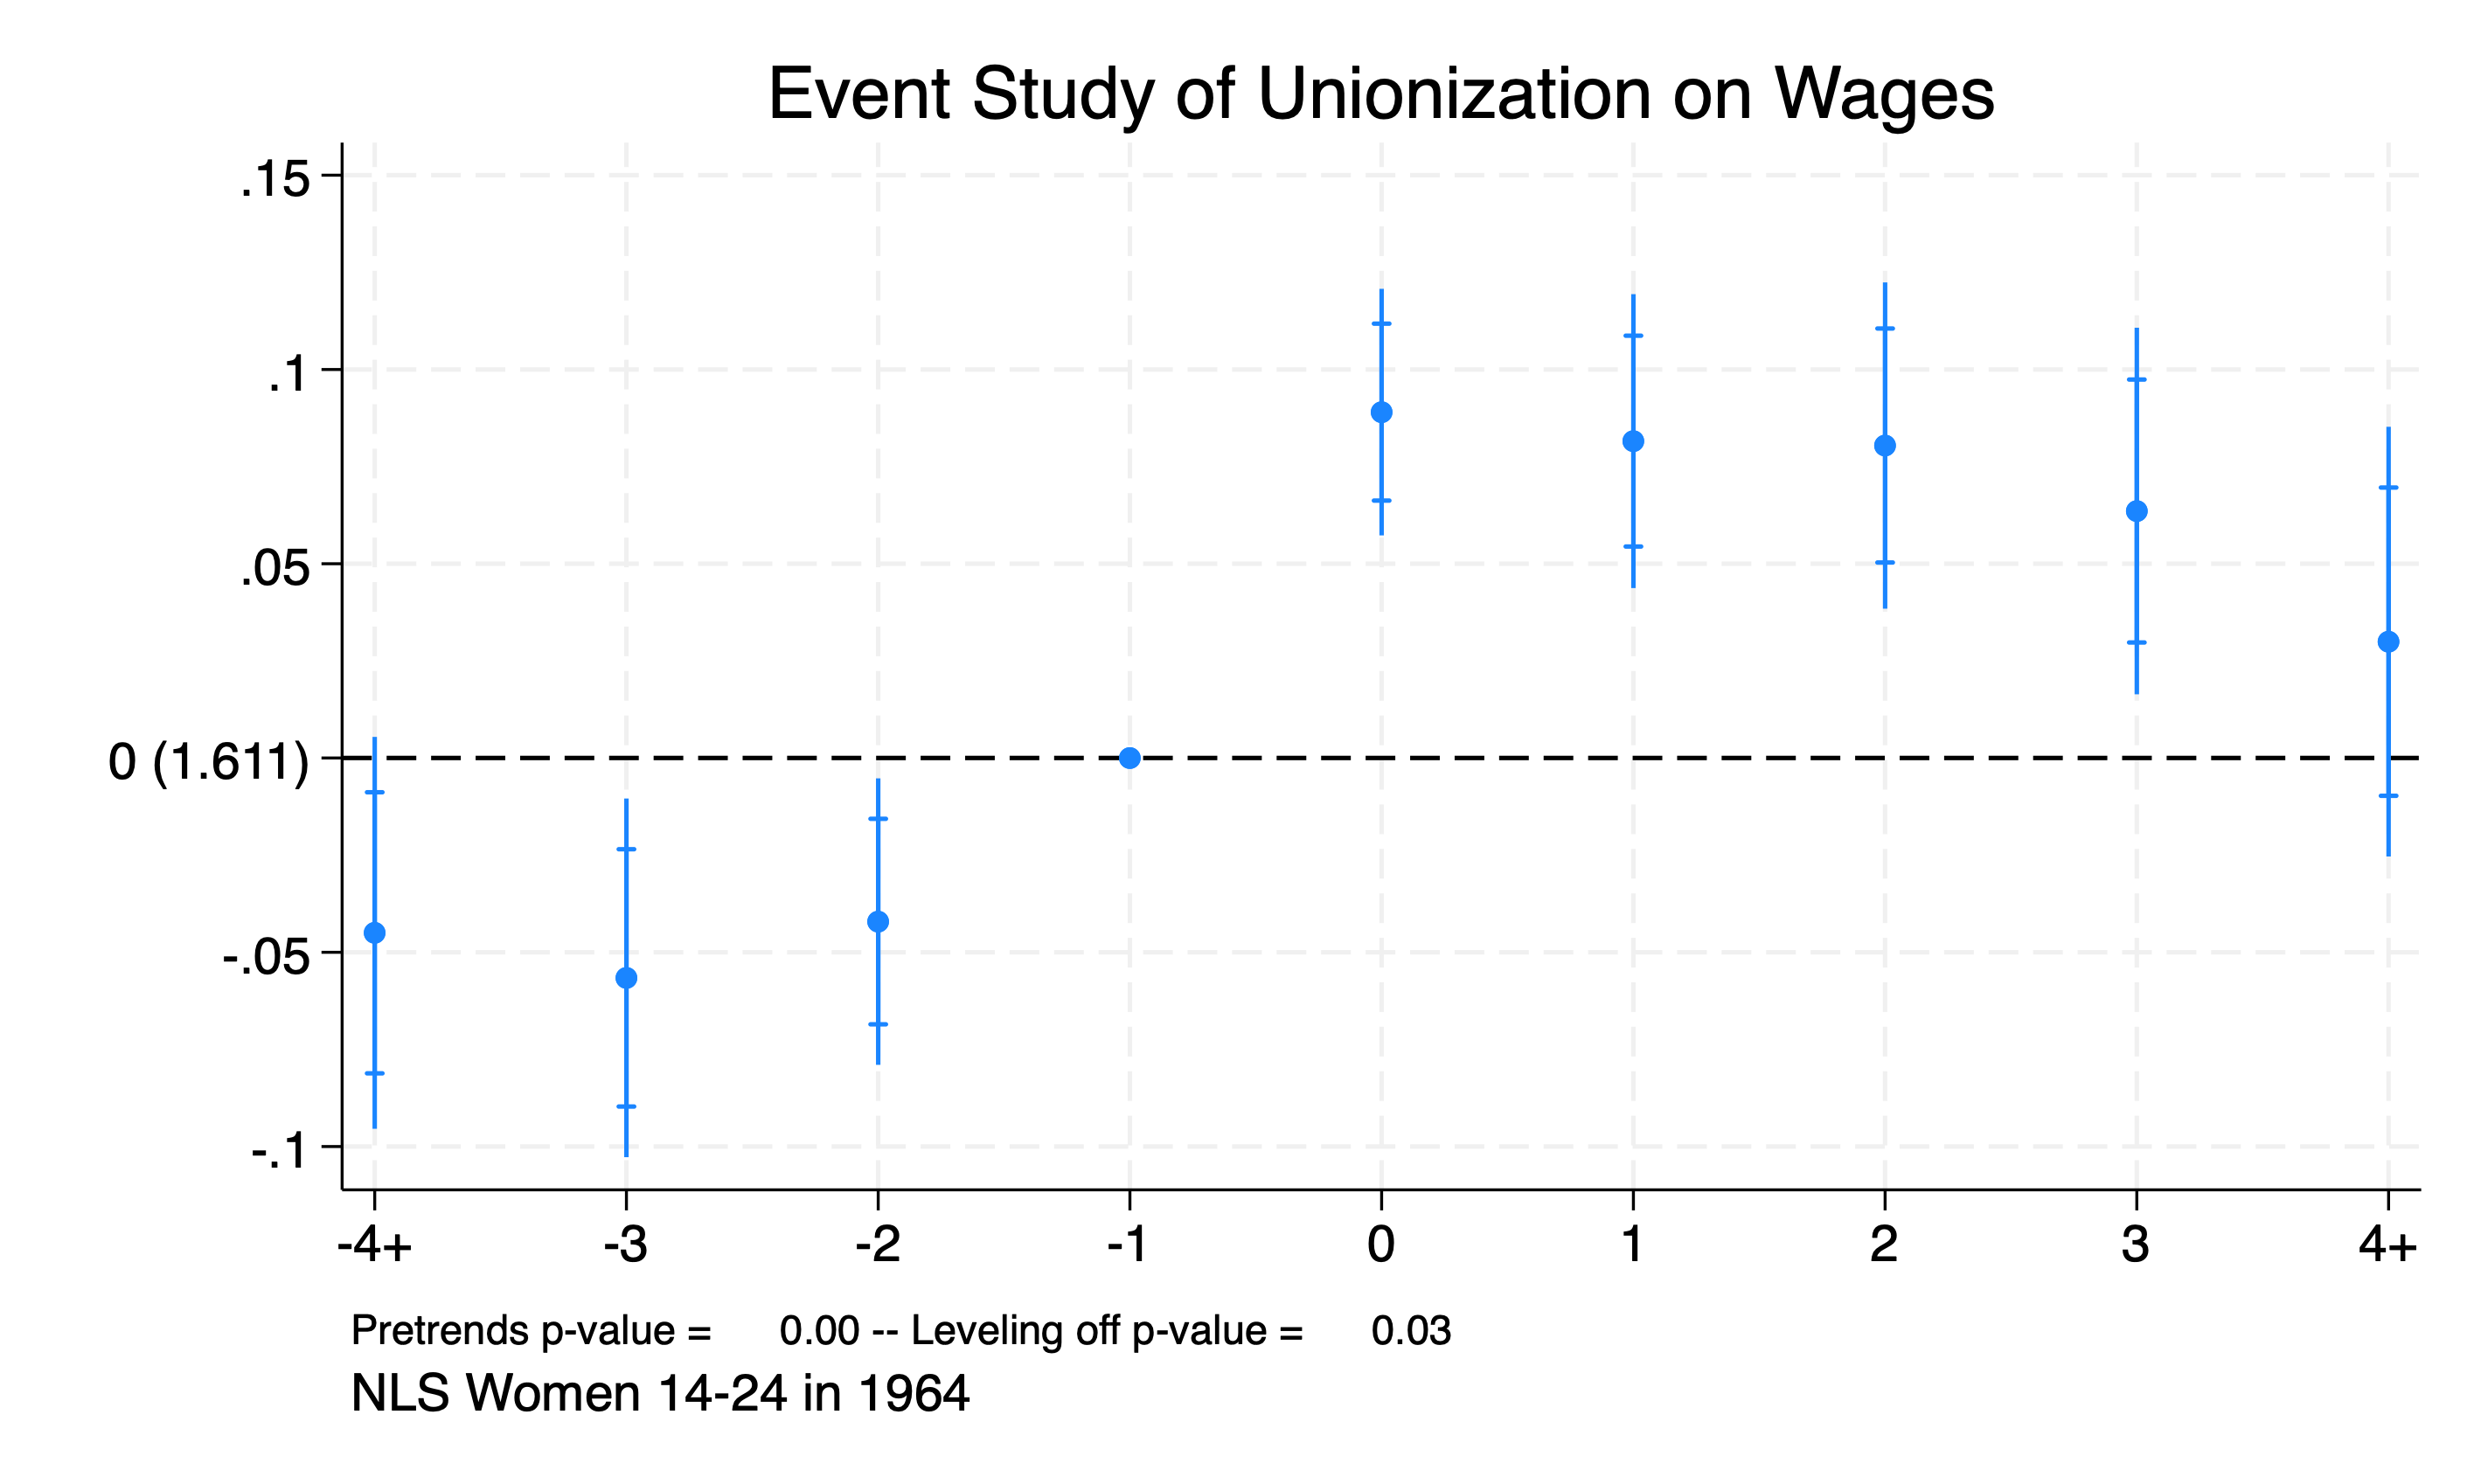
\includegraphics[keepaspectratio,alt={Event Study with 3 years pretreatment}]{ES2.png}}
\caption{Event Study with 3 years pretreatment}
\end{figure}

From our plot, we can easily see that we reject the null hypothesis that our pretreatment parameters are equal to 0.

We will run it with a window of 10 years for pretreatment.

\begin{Shaded}
\begin{Highlighting}[]
\NormalTok{xtevent ln\_w age c.age\#c.age ttl\_exp c.ttl\_exp\#c.ttl\_exp tenure , pol(union2) }\FunctionTok{w}\NormalTok{(10) }\KeywordTok{cluster}\NormalTok{(idcode) }\KeywordTok{impute}\NormalTok{(nuchange)}

\NormalTok{xteventplot, }\BaseNTok{title}\NormalTok{(}\StringTok{"Event Study of Unionization on Wages"}\NormalTok{) }\BaseNTok{caption}\NormalTok{(}\StringTok{"NLS Women 14{-}24 in 1964"}\NormalTok{)}
\end{Highlighting}
\end{Shaded}

\begin{figure}
\centering
\pandocbounded{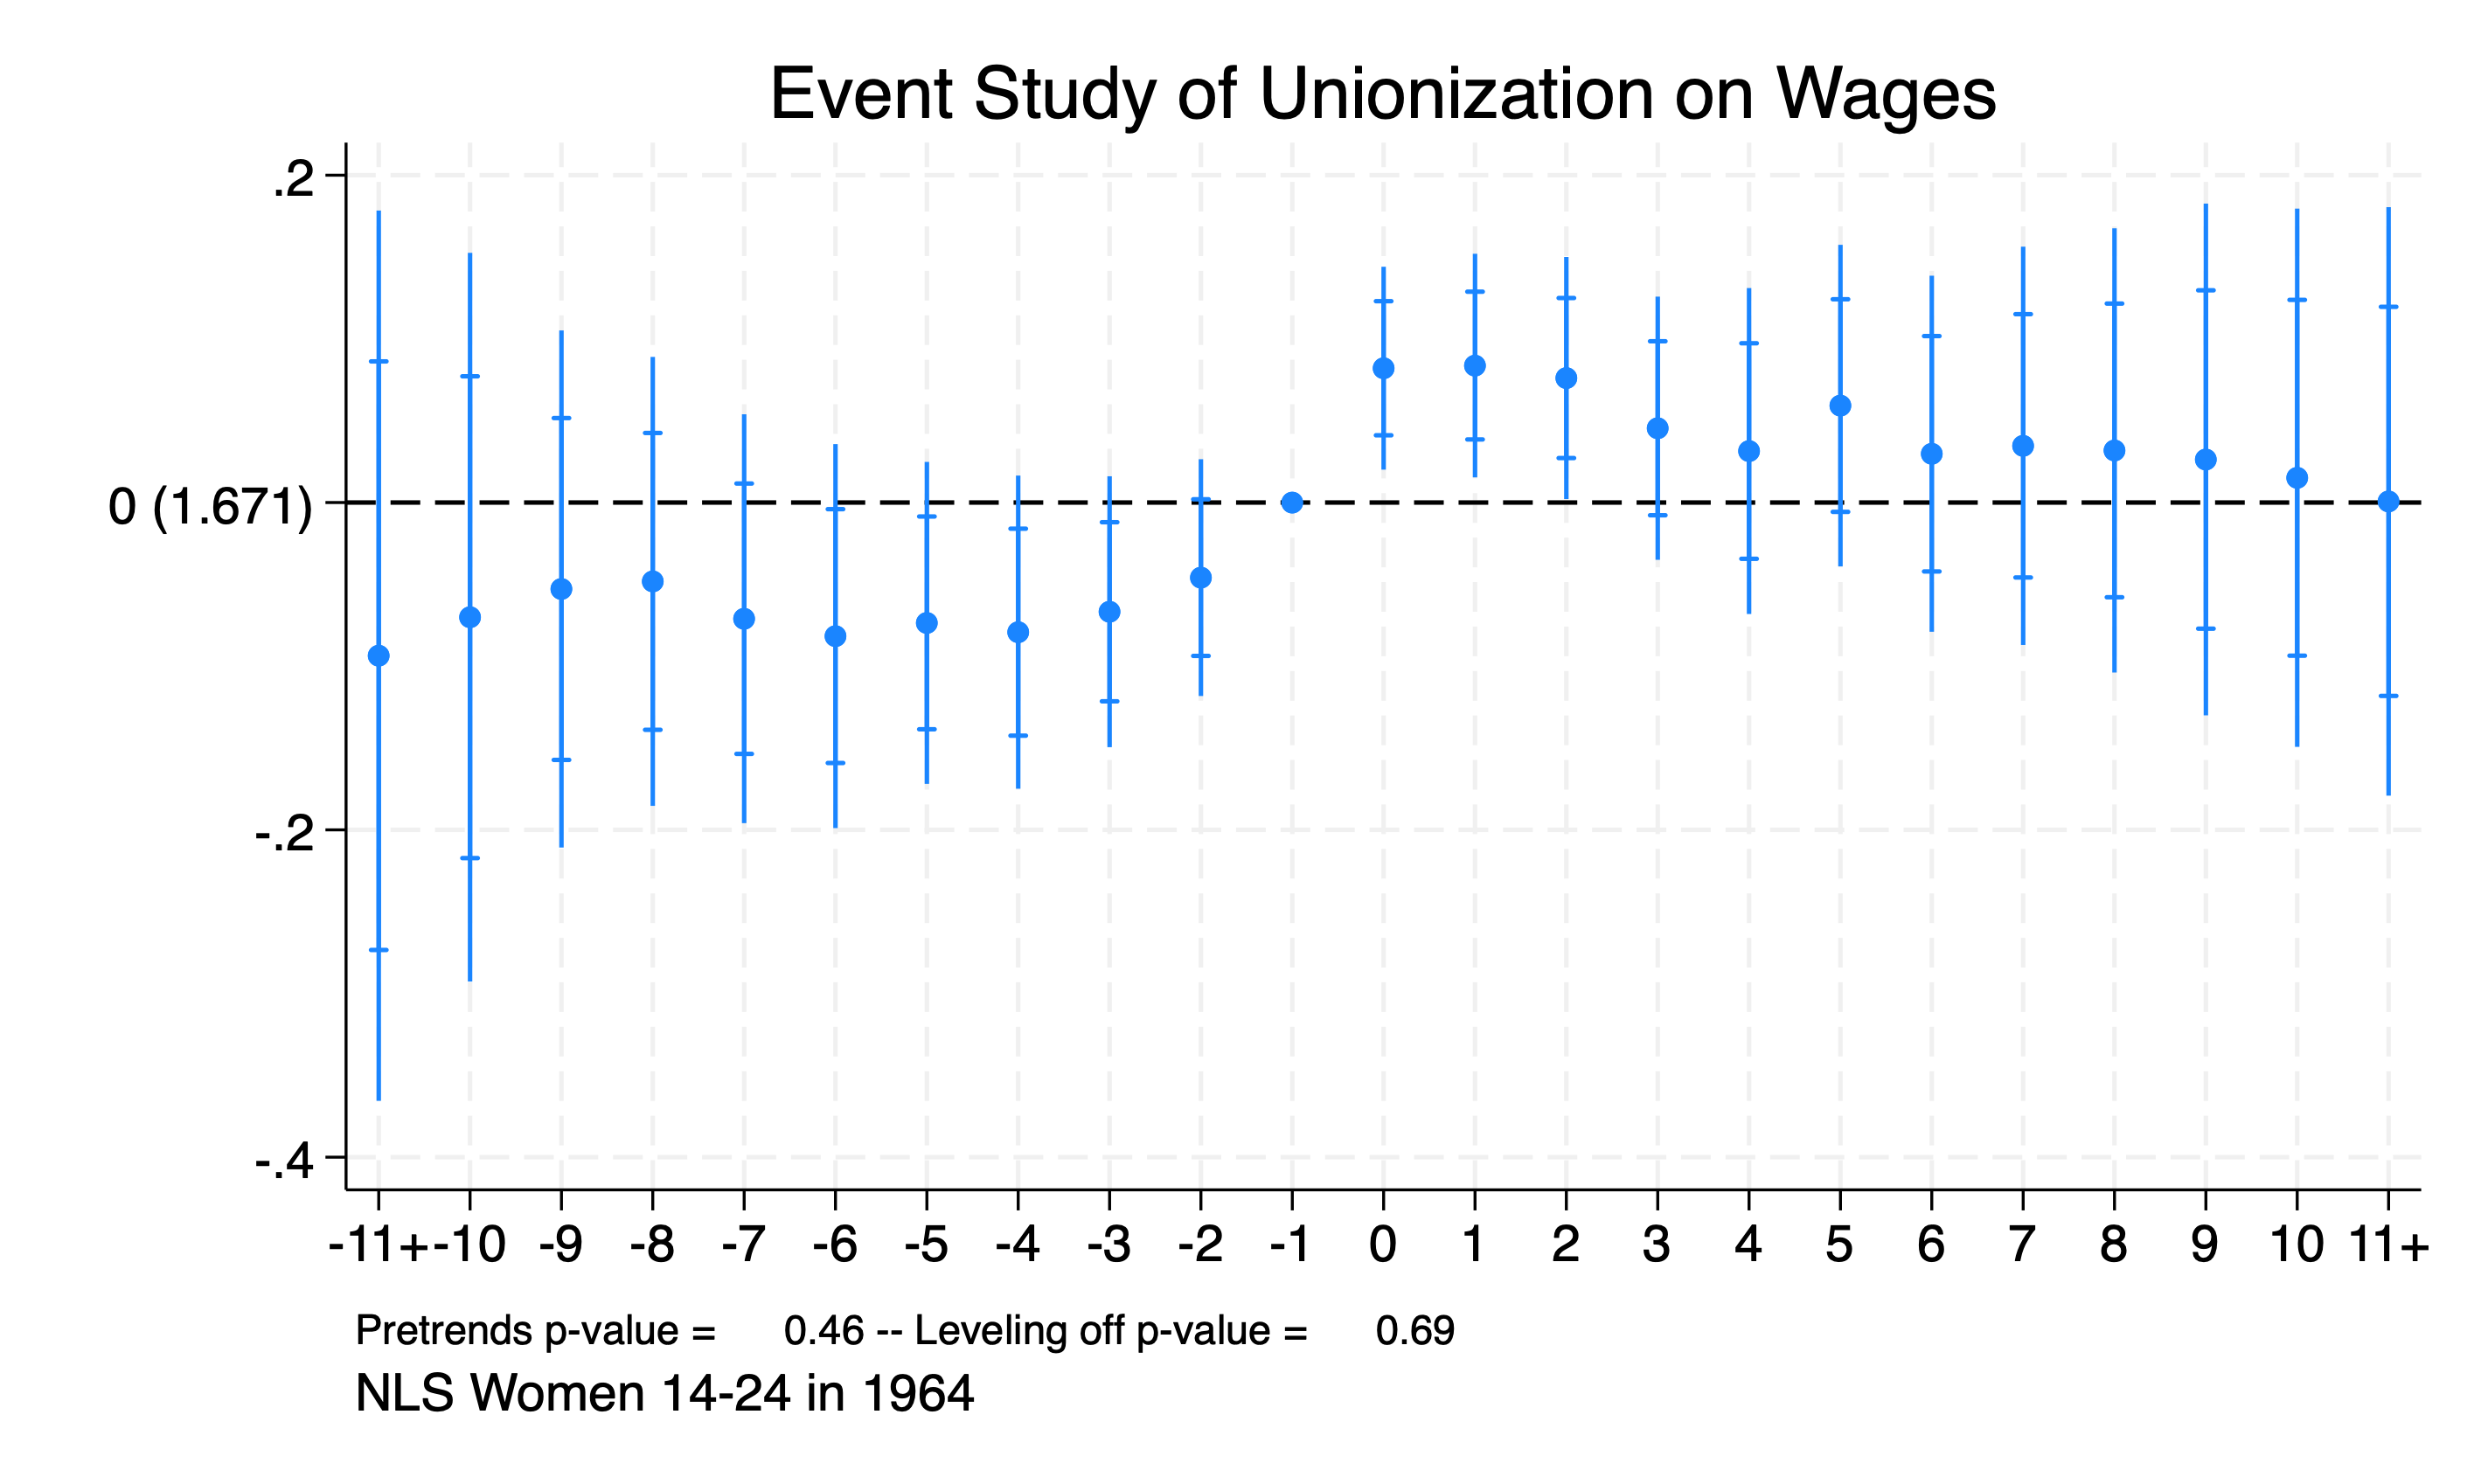
\includegraphics[keepaspectratio,alt={Event Study with 10 years pretreatment}]{ES3.png}}
\caption{Event Study with 10 years pretreatment}
\end{figure}

Our plot shows that we reject the null hypothesis for the pretreatment years 3-5. We need to be concerned that the parallel trends assumption does not hold.

\section{\texorpdfstring{\emph{xteventtest}}{xteventtest}}\label{xteventtest}

We can test the null hypothesis that the cumulative pretreatment variables are equal to 0 with the command \emph{xteventtest} command. We can add the options \emph{allpre} and \emph{allpre cumul} to test our pretreatment trends.

These conduct \(F\)-tests to test the joint exclusion restriction, which is similar to what we did in Econ 645.

We'll use the 3-year pretreatment window.

\begin{Shaded}
\begin{Highlighting}[]
\KeywordTok{quietly}\NormalTok{ xtevent ln\_w age c.age\#c.age ttl\_exp c.ttl\_exp\#c.ttl\_exp tenure , pol(union2) }\FunctionTok{w}\NormalTok{(3) }\KeywordTok{cluster}\NormalTok{(idcode) }\KeywordTok{impute}\NormalTok{(nuchange)}
\NormalTok{xteventtest, allpre }\KeywordTok{cumul}
\end{Highlighting}
\end{Shaded}

\begin{verbatim}
Test for all pre-event coefficients = 0

Test sums of coefficients

 ( 1)  _k_eq_m4 + _k_eq_m3 + _k_eq_m2 = 0

       F(  1,  2770) =   12.11
            Prob > F =    0.0005
\end{verbatim}

Our results from the \(F\)-test show that we reject the null hypothesis that the cumulative pretreatment trend is 0.

We'll test this for the 10-year pretreatment window.

\begin{Shaded}
\begin{Highlighting}[]
\KeywordTok{quietly}\NormalTok{ xtevent ln\_w age c.age\#c.age ttl\_exp c.ttl\_exp\#c.ttl\_exp tenure , pol(union2) }\FunctionTok{w}\NormalTok{(10) }\KeywordTok{cluster}\NormalTok{(idcode) }\KeywordTok{impute}\NormalTok{(nuchange)}
\NormalTok{xteventtest, allpre }\KeywordTok{cumul}
\end{Highlighting}
\end{Shaded}

\begin{verbatim}
Test for all pre-event coefficients = 0

Test sums of coefficients

 ( 1)  _k_eq_m11 + _k_eq_m10 + _k_eq_m9 + _k_eq_m8 + _k_eq_m7 + _k_eq_m6 +
       _k_eq_m5 + _k_eq_m4 + _k_eq_m3 + _k_eq_m2 = 0

       F(  1,   509) =    4.42
            Prob > F =    0.0360
\end{verbatim}

Again, our results from the \(F\)-test show that we reject the null hypothesis that the cumulative pretreatment trend is 0.

Cunningham, S. (2021). \emph{Causal Inference: The Mixtape}. Yale University Press.

Freyaldenhoven, S., Hansen C. \& Perez, JEP., and Shapiro J. (2021). \emph{XTEVENT: Stata module to estimate and visualize linear panel event-study models}. Statistical Software Components S458987, Boston College Department of Economics, revised 12 Jul 2024. \url{https://ideas.repec.org/c/boc/bocode/s458987.html}

Gruber, Levine, and Staiger (1999).Gruber, J., Levine, P.B., and Staiger,D. (1999). Abortion Legalization and Child Living Circumstances: Who Is the `Marginal Child'? \emph{The Quarterly Journal of Economics 114 (1)}: 263--91.

Huber, M. (2023). \emph{Causal Analysis: Impact Evaluation and Causal Machine Learning with Applications in R}. The MIT Press.

Huntington-Klein, N. (2022). \emph{The Effect: An Introduction to Research Design and Causality}. CRC Press.

Levitt, S.D. (2004). Why Crime Fell in the 1990s: Four Factors That Explain the Decline and Six That Do Not. \emph{Journal of Economic Perspectives 18 (1)}: 163-190

Princeton (2026). \emph{Difference-in-Differences in Stata: A step-by-step guide.} \url{https://libguides.princeton.edu/stata-did/1\#s-lg-box-wrapper-41689126}

\bibliography{book.bib,packages.bib}

\end{document}
